% Created by Bonita Graham
% Last update: December 2019 By Kestutis Bendinskas

% Authors: 
% Please do not make changes to the preamble until after the solid line of %s.

\documentclass[10pt]{article}
\usepackage[explicit]{titlesec}
\setlength{\parindent}{0pt}
\setlength{\parskip}{1em}
\usepackage{hyphenat}
\usepackage{ragged2e}
\RaggedRight

% These commands change the font. If you do not have Garamond on your computer, you will need to install it.
\usepackage{garamondx}
\usepackage[T1]{fontenc}
\usepackage{amsmath, amsthm}
\usepackage{graphicx}

% This adjusts the underline to be in keeping with word processors.
\usepackage{soul}
\setul{.6pt}{.4pt}


% The following sets margins to 1 in. on top and bottom and .75 in on left and right, and remove page numbers.
\usepackage{geometry}
\geometry{vmargin={1in,1in}, hmargin={.75in, .75in}}
\usepackage{fancyhdr}
\pagestyle{fancy}
\pagenumbering{gobble}
\renewcommand{\headrulewidth}{0.0pt}
\renewcommand{\footrulewidth}{0.0pt}

% These Commands create the label style for tables, figures and equations.
\usepackage[labelfont={footnotesize,bf} , textfont=footnotesize]{caption}
\captionsetup{labelformat=simple, labelsep=period}
\newcommand\num{\addtocounter{equation}{1}\tag{\theequation}}
\renewcommand{\theequation}{\arabic{equation}}
\makeatletter
\renewcommand\tagform@[1]{\maketag@@@ {\ignorespaces {\footnotesize{\textbf{Equation}}} #1.\unskip \@@italiccorr }}
\makeatother
\setlength{\intextsep}{10pt}
\setlength{\abovecaptionskip}{2pt}
\setlength{\belowcaptionskip}{-10pt}

% control floats
%% \renewcommand\floatpagefraction{.9}
%% \renewcommand\topfraction{.9}
%% \renewcommand\bottomfraction{.9}
%% \renewcommand\textfraction{.2}
%% \setcounter{totalnumber}{50}
%% \setcounter{topnumber}{50}
%% \setcounter{bottomnumber}{50}


% These commands set the paragraph and line spacing
\titleformat{\section}
  {\normalfont}{\thesection}{1em}{\MakeUppercase{\textbf{#1}}}
\titlespacing\section{0pt}{0pt}{-10pt}
\titleformat{\subsection}
  {\normalfont}{\thesubsection}{1em}{\textit{#1}}
\titlespacing\subsection{0pt}{0pt}{-8pt}
\renewcommand{\baselinestretch}{1.15}

% This designs the title display style for the maketitle command
\makeatletter
\newcommand\sixteen{\@setfontsize\sixteen{17pt}{6}}
\renewcommand{\maketitle}{\bgroup\setlength{\parindent}{0pt}
\begin{flushleft}
\sixteen\bfseries \@title
\medskip
\end{flushleft}
\textit{\@author}
\egroup}
\makeatother

% This styles the bibliography and citations.
%\usepackage[biblabel]{cite}
\usepackage[sort&compress]{natbib}
\setlength\bibindent{2em}
\makeatletter
\renewcommand\@biblabel[1]{\textbf{#1.}\hfill}
\makeatother
\renewcommand{\citenumfont}[1]{\textbf{#1}}
\bibpunct{}{}{,~}{s}{,}{,}
\setlength{\bibsep}{0pt plus 0.3ex}




%%%%%%%%%%%%%%%%%%%%%%%%%%%%%%%%%%%%%%%%%%%%%%%%%

% Authors: Add additional packages and new commands here.  
% Limit your use of new commands and special formatting.

\usepackage{physics} % for \dd
\usepackage{hyperref}

\usepackage{xcolor}
\newcommand{\jy}[1]{\textcolor{blue}{JY: #1}}
\newcommand{\eds}[1]{\textcolor{red}{EDS: (#1)}}
\newcommand{\mc}[1]{\textcolor{orange}{MC: (#1)}}

% Place your title below. Use Title Capitalization.
\title{On Sample Size Needed for Block Bootstrap Confidence Intervals
  to Have Desired Coverage Rates}

% Add author information below. Communicating author is indicated by an 
% asterisk, the affiliation is shown by superscripted lower case letter if 
% several affiliations need to be noted.
\author{
Mathew Chandy*$^{a}$, Elizabeth D. Schifano$^{a}$, Jun Yan$^{a}$ \\ \medskip 
$^{a}$Department of Statistics, University of Connecticut, Storrs, CT \\ \medskip 
Student: mathew.chandy@uconn.edu* \\
Mentors: elizabeth.schifano@uconn.edu, jun.yan@uconn.edu
}
\pagestyle{empty}
\begin{document}

% Makes the title and author information appear.
\vspace*{.01 in}
\maketitle
\vspace{.12 in}

% Abstracts are required.
\section*{abstract}
Block bootstrap is widely used in constructing confidence intervals for 
parameters estimated from stationary time series. Theoretically, the method
should provide valid confidence intervals as the length of the time series goes
to infinity. In practice, however, it is necessary to know 
how large of a finite 
sample is required for block bootstrap confidence intervals to work well. This 
study aims to answer this question in a simple simulation setting where the data 
are generated from a first-order autoregressive process. The empirical coverage 
rates of several commonly used bootstrap confidence intervals for the mean, 
standard deviation, and the lag-1 autocorrelation coefficient are compared. A 
quite large sample is found necessary for the intervals to have the right 
coverage rates even when estimating a simple parameter like the mean. Some block 
bootstrap methods could fail when estimating the lag-1 autocorrelation. It is 
surprising that the coverage property even deteriorates as the sample size 
increases with some commonly used block bootstrap confidence intervals including 
the percentile intervals and bias-corrected intervals.

% Keywords are required.
\section*{keywords} 
% List Eight to Ten Capitalized Keywords Separated by \ul{Semicolons}; Do Not Use Period at The End
Autocorrelation; Bias-Correction; Centering; Dependent Data; Percentile; 
Resampling; Simulation; Time Series  


\vspace{.12 in}

% Start the main part of the manuscript here.
% Comment out section headings if inappropriate to your discipline.
% If you add additional section or subsection headings, use an asterisk * to avoid numbering. 


\section*{introduction}

Block bootstrap is a tool to construct confidence intervals (CI) to make
inferences about dependent data. Essentially, it depends on correct estimation
of the uncertainty in the estimation, similar to the standard bootstrap 
\citep{efron1979bootstrap}, but for serially dependent data.
Early ideas of block bootstrap were developed not long after the standard 
bootstrap.\citep{hall1985resampling, carlstein1986use,kunsch1989jackknife} It 
has since
been applied in various fields, for instance, econometrics and 
meteorology.\citep{mackinnon2006bootstrap, varga2017generalised}
Block bootstrap is especially useful for serially dependent data when the serial 
dependence is not specified or not of primary interest. The method is expected 
to produce CIs with coverage rates matching their nominal levels as the sample 
size grows. However, when dealing with finite sample sizes, an important 
question is how large the sample size must be for block bootstrap CIs to have 
the desired coverage rates.
%\eds{I think the superscript citations need to go before the punctuation.  
%Please check in other AJUR papers and adjust throughout the paper if needed.}
%\mc{from the style guide: "Please bold and superscript the numbers for 
%references in the text.1 Separate superscripted numbers by comma and space,1, 2 
%they should be separated by an en-dash if the consecutive list of more than two 
%numbers is used.1–3 List them AFTER punctuation (be it comma or period) with no 
%space.2} 
%\eds{thank you for checking!}

\citet{lahiri1999theoretical} finds that moving block bootstrap has better 
performance than non-overlapping block bootstrap. Additionally, moving block 
bootstrap with nonrandom
block sizes results in lower mean-squared errors than moving block bootstrap
with random block sizes. \citet{buhlmann1999block} notes that a drawback of 
block bootstrap is that it heavily depends on block size, which has to be chosen
by the user of the method.
Even when using the appropriate settings, as noted by
\citet{buhlmann2002bootstraps} observes some general drawbacks of block 
bootstrap --- with respect to how reasonably it imitates the data-generating 
process. In addition, although block bootstrap is primarily used for stationary 
time series, it can be outperformed by other bootstrap schemes for linear time
series and categorical processes. Still, \citet{buhlmann2002bootstraps}
emphasizes that a significant advantage of block bootstrap is its simplicity.
To be more specific, the resampling step of block bootstrap is not 
computationally more difficult than the resampling step of basic bootstrap.
Furthermore, block bootstrap performs better than local bootstrap in terms of
mimicking dependence structures.

\eds{If we include all these drawbacks here, we need to also provide some good 
features of block bootstrap as well, otherwise, why do we care about their CI 
performance?}
\mc{addressed}

For independent data, extensive research has explored the effectiveness of
bootstrap standard errors in providing accurate uncertainty measures. For 
example, \citet{hesterberg2015teachers} observes that while percentile-based CIs 
for the mean parameter are more accurate than $t$-intervals for larger sample 
sizes, their accuracy diminishes for smaller sample sizes. The optimal parameter 
estimation of a distribution, according to \citet{chernick2009revisiting}, 
depends on the sample size, the number of bootstrap replicates, and the 
confidence level. In structural equation modeling, \citet{nevitt2001performance} 
find that a sample size of 200--1000 is sufficient for interval estimation using 
standard nonparametric bootstrap. In estimating variance components, 
\citet{burch2012nonparametric} reports that as the sample size increases under a 
normal distribution, nonparametric bootstrap methods approach the coverage of a 
pivotal quantity, but for other distributions, the coverage can deteriorate. In 
estimating the correlation coefficient of bivariate normal data, 
\citet{puth2015variety} note that even for a sample size of~$100$ with true 
correlation coefficient~0, bootstrap methods are less accurate than the Fisher's 
transformation. The prevailing consensus highlights the necessity of a 
substantial sample size for bootstrap CIs to attain the desired coverage.


Limited research has offered practical guidance concerning the requisite sample
size for employing block bootstrap inference with dependent data. In the context 
of linear regression involving dependent data, where regression errors stem from 
a homoscedastic autoregressive process of order-1, the investigation conducted 
by \citet{goncalves2005bootstrap} reveals that, in cases of small sample sizes, 
standard error estimates derived from the moving block bootstrap approach may 
demonstrate greater accuracy than those based on closed-form asymptotic 
estimates. Nonetheless, even when considering a substantial sample size of 
~$1024$, confidence intervals generated through the moving block bootstrap 
method still fail to adequately encompass the target parameter. The scarcity of 
existing literature addressing the necessary sample sizes conducive to the 
efficacy of block bootstrap techniques has spurred the initiation of the present 
study.


The goal of this paper is to provide recommendations on necessary sample size 
for block bootstrap with dependent data, similar to what was done for basic 
bootstrap in \citet{hesterberg2015teachers}. We consider a simple situation of 
a stationary time series, where the parameters of interests are the mean, 
standard deviation, and the first-order autocorrelation coefficient. We compare 
six variants of block bootstrap CIs from the 
literature:\citep{diciccio1996bootstrap, rice2006mathematical} a standard normal 
CI, a 
Student's $t$ CI, a percentile CI, a bias-corrected CI, a bias-corrected and 
accelerated CI, and a recentered percentile CI proposed in this article. Their 
empirical coverage rates at different sample sizes and dependence levels are 
compared in a simulation study. The results of this study suggest that recovery 
of temporal dependence parameters is reliant on the type of interval used.



The remainder of the paper is organized as follows. The first section 
reviews block bootstrap procedures and how to use block bootstrap estimates to
construct CIs; a simple CI obtained by recentering at the original point 
estimate is proposed for comparison. The second section reports a simulation 
study comparing the coverage rates of six block bootstrap CIs. A discussion
concludes in the final section.

\section*{block bootstrap cis}
\label{sec:bbci}

Consider a stationary time series $\{X_t: t = 1, \ldots, n\}$ with length~$n$. 
Our goal is to construct a CI for a parameter $\theta$ in the data generating 
model of the series. Suppose that $\hat\theta_n$ is a point estimator 
of~$\theta$ based on the observed series. Bootstrap is a powerful approach to
construct CIs. If the observations in the series were independent, a standard
nonparametric bootstrap procedure would draw a large number~$B$ bootstrap copies 
of the observed data, and calculate a bootstrap point estimate 
$\hat\theta_n^{(b)}$ for each copy $b = 1, \ldots, B$. The uncertainty of 
$\hat\theta_n$ is then estimated by the empirical uncertainty of the bootstrap 
point estimates. When serial dependence is present, the bootstrap procedure 
needs to preserve the serial dependence. Block bootstrap was motivated for this 
situation. 

\subsection*{Block Bootstrap}

Block bootstrap preserves the serial dependence in the observed data by 
partitioning the data into blocks and performing bootstrap on the blocks. In
particular, consider block size~$l$ and, for convenience, suppose that $n$ is a 
multiple of $l$ such that there are $k = n / l$ blocks. Each block~$j$ is
$Y_j = \{X_{(j - 1) l + 1}, \ldots, X_{(j - 1) l + l}\}$, $j = 1, \ldots, k$.
Then, we sample $k$ blocks of $Y_j$'s from the set $\{Y_1, \ldots, Y_k\}$ with
replacement and concatenate the $k$ sampled blocks in the order they are picked 
to form a bootstrap sample of the data. The formation of the bootstrap sample 
ensures that the between-block dependence is weak and that the within-block 
serial dependence is preserved. Because the blocks here are non-overlapping, 
this bootstrap approach is known as non-overlapping block bootstrap, or simple 
block bootstrap.


Alternatively, block-bootstrap can be done with overlapping or moving blocks.
Define moving blocks
\[
Z_j = \{X_j, \ldots, X_{j + l - 1}\}, \quad 
j = 1, \ldots, n - l + 1.
\]
Now we draw $k$ blocks from the $(n - l + 1)$ blocks 
of $Z_j$'s with replacement and then align them in the order they were picked to 
form a block bootstrap sample. If $n$ is not a multiple of~$l$, the last block 
selected will be reduced in size so that the final size of the block bootstrap 
sample is $n$. It is also possible to implement moving block bootstrap while 
allowing blocks to wrap around the end of the series. In other words, define 
moving blocks (assuming $l > 1$) as:
\begin{equation*}
Z_j =
    \begin{cases}
        \{X_j, \ldots, X_{j + l - 1}\}, & \text{if } j = 1, \dots, n - l + 1,\\
        \{X_j, \ldots, X_n, X_1, \ldots, X_{j-n+l-1}\}, & \text{if } j = n - l
        + 2 ,\dots, n.
    \end{cases}
\end{equation*}
This version does not require that $n/l$ be an integer.


The block size~$l$ needs to be chosen with care. It should be large enough for
each bootstrap sample to preserve the serial dependence, yet small enough for
there to be a large number of blocks to give sufficient variability between each 
bootstrap sample. As $n$ increases, both~$l$ and $n / l$ should also increase. 
To achieve this, the order of $l$ is often assigned a value as a function of 
$n$. A common 
expression that is considered optimal for the order of $l$ is 
$\lceil n^{1/3} \rceil$,
\citep{buhlmann1999block} 
which was adopted in this study.

\subsection*{Block Bootstrap CIs}

Suppose that we have repeated the steps in the last subsection $B$ times, and
that for $b \in \{1, \ldots, B\}$, we have obtained a bootstrap point estimate
$\hat\theta_n^{(b)}$ based on the $b$th bootstrap sample using the same method
that was applied to $\{X_t: t = 1, \ldots, n\}$ to obtain $\hat\theta_n$. Now
the question is how to construct a CI for $\theta$ using the $B$ bootstrap point 
estimates $\{\hat\theta_n^{(1)}, \ldots, \hat\theta_n^{(B)}\}$. We consider six 
kinds of block bootstrap CIs adapted from standard bootstrap CIs.


\paragraph{Standard Normal CI}
Assuming that $\hat\theta_n$ is asymptotically normally distributed with 
$\theta$ as the mean, we just need an estimate of the standard error to 
construct an approximate CI.\citep{efron1993introduction} Let
$\widehat{\text{SE}}$ be the empirical standard error of the bootstrap point 
estimates $\hat\theta_n^{(b)}$ for $b \in \{1, \ldots, B\}$. Let $z_{(\alpha)}$ 
be the quantile function $F^{-1}(\alpha)$ of the standard normal distribution. 
A $(1 - \alpha)100\%$ standard normal CI is
\[
(\hat{\theta}_{n} - z_{(1-\alpha/2)}\widehat{\text{SE}}, \quad
\hat{\theta}_{n} - z_{(\alpha/2)}\widehat{\text{SE}}).
\]
%\eds{If $z_{(\alpha)}$ is the upper quantile, then $z_{(\alpha/2)}$ will be 
%positive and $z_{(1-\alpha/2)}$ will be negative for small $\alpha$ values; with
%the subtraction of the quantiles, the smaller CI endpoint would appear to
%be listed first.  Please check this notation, and the notation for Student's $t$ 
%CI, and other intervals which use the $z_{(\alpha)}$ upper standard normal 
%quantile.} 
%\mc{Replaced upper quantile with quantile function}

This CI is centered by the original point estimate $\hat\theta_n$ and is 
symmetric. The standard CI is classified by \citet{efron1993introduction} 
as a confidence interval based on bootstrap ``tables". Its 
validity relies on whether the distribution of $\hat\theta_n$ is reasonably well 
approximated by its asymptotic normal distribution and whether the bootstrap
$\widehat{\text{SE}}$ approximates the true standard error.


\paragraph{Student's $t$ CI}
The procedure for constructing a Student's $t$ CI based on standard bootstrap is 
described in \citet{efron1993introduction}. Let $t_{(\alpha, k)}$ be the 
quantile function $F^{-1}(\alpha, k)$ of a $t$ distribution with $k$ degrees of 
freedom. With 
block bootstrapping, 
a $(1 - \alpha)100\%$ Student's $t$ CI is
\[
(\hat{\theta}_{n} - t_{(1-\alpha/2), k - 1}\widehat{\text{SE}}, \quad
\hat{\theta}_{n} - t_{(\alpha/2), k -1}\widehat{\text{SE}}),
\]
%\eds{define $t_{(.)}$ and check the signs}  \mc{addressed}
where $k$ is the number of blocks. This CI is centered by the original point 
estimate $\hat\theta_n$ and is symmetric. Like the standard normal interval, the
Student's $t$ CI is classified by \citet{efron1993introduction} 
as a confidence interval based on bootstrap ``tables". In this case, its 
validity relies on whether the distribution of $\hat\theta_n$ is reasonably well 
approximated by the $t_{k-1}$ distribution with an expected value of $\theta$ 
and whether the bootstrap $\widehat{\text{SE}}$ approximates the true standard 
error.


\paragraph{Percentile CI}
The percentile CI was first suggested in \citet{efron1979bootstrap}.
Let $\hat\theta_{n, \alpha}^B$ be the empirical $100\alpha$th percentile of
$\{\hat\theta_n^{(1)}, \ldots, \hat\theta_n^{(B)}\}$. 
A $(1 - \alpha)100\%$ empirical percentile CI is
\[
(\hat\theta_{n, \alpha/2}^{B}, \quad \hat\theta_{n, 1 - \alpha/2}^{B}).
\]
This CI is not necessarily centered by the original point estimate 
$\hat\theta_n$. As will be shown in our simulation study, this approach works 
well for the marginal mean and standard deviation of a serially dependent 
process, but its coverage of the temporal dependence deteriorates as $n$ 
increases, which is contrary to what one would expect.


\paragraph{Bias-Corrected (BC) CI}
The procedure for constructing a bias-corrected Bootstrap CI based on standard
bootstrap is described in \citet{carpenter2000bootstrap}. Let
$\hat{z}_0 = \Phi^{-1}\{\#\{\hat\theta_n^{(b)} < \hat{\theta}_n\} / B\}$ for
$b \in \{1, \ldots, B\}$. Define 
$\alpha_1 = \Phi(2\hat{z}_0 - z_{1 - \alpha/2})$ 
and $\alpha_2 = \Phi(2\hat{z}_0 - z_{\alpha/2})$. 
A $(1 - \alpha)100\%$ ~BC CI is
\[
(\hat\theta_{n, \alpha_1}^{B}, \quad \hat\theta_{n, \alpha_2}^{B}).
\]
%\eds{the $z_{\alpha/2}$ and $z_{1 - \alpha/2}$ may need to be switched now in 
%$\alpha_1$ and $\alpha_2$ with the quantile definition for $z_{\alpha}$ -- 
%please check.} 
%\mc{yes they had to be switched}

\paragraph{Bias-Corrected and Accelerated (BCA) CI}
The BCA CI was first suggested in \citet{efron1987better}. Let $Z_{(i)}$ be the 
original sample without the $i$th block $z_i$ for $i \in \{1, \ldots, k\}$, let 
$\hat{\theta}_{(i)}$ be the statistic of $Z_{(i)}$, and let 
$\hat{\theta}_{(.)} = k^{-1}\sum_{i=1}^{k} \hat{\theta}_{(i)}$. 
Let
\begin{equation*}
\hat{a} = \frac{\sum_{i=1}^{k} (\hat{\theta}_{(.)} -
  \hat{\theta}_{(i)})^3}{6\{\sum_{i=1}^{k} (\hat{\theta}_{(.)} -
  \hat{\theta}_{(i)})^2\}^{3/2}}.
\end{equation*}
Define
\begin{equation*}
\alpha_1 = \Phi\left(\hat{z}_{0} + \frac{\hat{z}_{0} +
  z_{\alpha/2}}{1 - \hat{a}(\hat{z}_{0} + z_{\alpha/2})}\right)
\end{equation*}
and
\begin{equation*}
\alpha_2 = \Phi\left(\hat{z}_{0} + \frac{\hat{z}_{0} +
  z_{1 - \alpha/2}}{1 - \hat{a}(\hat{z}_{0} + z_{1 - \alpha/2})}\right).
\end{equation*}
%\eds{please check $z_{\alpha/2}$ and $z_{1 - \alpha/2}$ in 
%$\alpha_1$ and $\alpha_2$ with the quantile definition for $z_{\alpha}$} 
%\mc{this one is okay}
A $(1 - \alpha)100\%$ ~BCA CI is
\[
(\hat\theta_{n, \alpha_1}^{B}, \quad \hat\theta_{n, \alpha_2}^{B}).
\]
This CI is not necessarily centered by $\hat\theta_n$. The BCA method corrects 
for bias and skewness of the $B$ bootstrap point estimates 
$\{\hat\theta_n^{(1)}, \ldots, \hat\theta_n^{(B)}\}$ by including 
bias-correction and acceleration factors. The acceleration factor refers to the 
rate of change of the standard error of $\hat\theta_n$ with respect to $\theta$.


\paragraph{Recentered Percentile CI}
We propose a CI that is centered at the original point estimate and uses the 
variation in the bootstrap estimates to construct the error bound. 
The motivation behind proposing such an interval was based on the 
simulation performance of the BC and BCA intervals, which will be discussed
further in the Results section. 
This interval 
requires
the computation of $\bar\theta_n^B = n^{-1}\sum_{b=1}^B \hat\theta_n^{(b)}$, the 
mean of all bootstrap point estimates. A $(1 - \alpha)100\%$ CI is
centered around $\hat\theta_n$ and can be written as 
\[
(\hat\theta_n + \hat\theta_{n, \alpha/2}^{B} - \bar\theta_n^{B}, \quad
\hat\theta_n + \hat\theta_{n, 1 - \alpha/2}^{B} - \bar\theta_n^{B}).
\]
It is not necessarily symmetric, as different critical values are used to 
compute the lower and upper bounds. It has the same width as the percentile CI.


\section*{simulation design}
\label{sec:simdes}

%\subsection*{Design}

\eds{We compared the performance of the different block bootstrap CI methods 
under two marginal distributions: normal and exponential.} 

\subsection*{Normal Marginal Distribution}
%We designed a simulation study to compare the performance of the different block 
%bootstrap CI methods. In particular, 
We generated time series $X_t$ from a 1st 
order autoregressive (AR(1)) process:
\begin{equation*}
X_t = \phi X_{t-1} + \epsilon_t,
\end{equation*}
where $\phi$ is an autoregressive coefficient, and $\epsilon_t$ is a series of
independent errors from a normal distribution with mean zero and variance
$\sigma_{\epsilon}^2$. The strength of the serial dependence is controlled by
$\phi$, which was set to five levels: $\{-0.4, -0.2, 0.0, 0.2, 0.4\}$. We only
used serial dependences as strong as 0.4, because we only seek to 
establish the 
general trend as the strength of the autocorrelation 
increases, and how it varies depending on the sign of the autocorrelation and 
the parameter of interest. The 
series $X_t$ has mean zero and variance 
$\sigma_x^2 = (1 - \phi^2) \sigma_{\epsilon}^2$, so for each value of $\phi$, we 
set $\sigma_{\epsilon}^2 = 1 / (1 - \phi^2)$ such that $\sigma_x^2 = 1$.


Three target parameters of $X_t$ were considered:
1) $\mu = 0$, the mean of $X_t$;
2) $\sigma_x = 1$, the standard deviation of $X_t$; and
3) $\phi$, the lag-1 autocorrelation coefficient.
To investigate the effect of sample size~$n$, we considered an array of values
$n \in \{100, 200, 400, 800, 1600, 3200\}$. In each configuration, we generated 
10000 replicates. The 
block bootstrap sampling step was done with function \texttt{tsboot} from R 
package \textsl{boot},\citep{boot} with block size $\lceil n / l \rceil$. This 
function by default is an implementation of moving block bootstrap as described 
in the previous section, meaning that that blocks are allowed to wrap around, 
and we tried both $l = \lceil n^{1/3} \rceil$ and $l = \lceil 2n^{1/3} \rceil$,
keeping the order of the block size constant but varying the coefficient. The
results for $l = \lceil 2n^{1/3} \rceil$ are included in the Appendix.
For each replicate, we constructed 
six 95\% block bootstrap 
CIs for each parameter as described in the last section with $B = 1000$. We can 
estimate $\mu$, 
$\sigma_x$, and $\phi$ by computing the sample mean, sample standard deviation, 
and lag-1 autocorrelation, respectively, of each bootstrap sample. Then we can 
construct intervals for each parameter using the appropriate procedures 
described in \textit{Block Bootstrap CIs}. 
Then we estimated their actual coverage 
rates along with their 95\% confidence intervals from the 10000 replicates. 


The coverage rates of the CIs were used to compare the performance of CIs. Let
$\hat\theta_{L, r}$ and $\hat\theta_{U, r}$ be the lower and upper bound,
respectively, for the confidence interval constructed for each replicate
$r \in \{1, \ldots, R\}$, where $R$ is the number of replicates. Then
$cov = \#\{\hat\theta_{L, r} < \theta < \hat\theta_{U, r} \}/R$, for
$r \in \{1, \ldots, R\}$. If a CI method is valid, then the coverage rate is
expected to match the nominal level. Because it is unlikely for the coverage to 
exactly match the nominal level, we can construct a 95\% Wald-type CI of the 
coverage rate 
(which is an estimate of a proportion with $R = 10000$). If the proportion 0.95 
is included in the interval, the block bootstrap method is likely performing 
well. If all values in the interval are below 0.95, the results would suggest 
that the method either is providing inaccurate estimation, is underestimating 
the process' variability, or a combination of both. If all values in the 
interval are above .95, the results suggest that the method is overestimating 
the process' variability. \citet{brown2001interval} notes that the Wald-type 
interval has poor coverage as the proportion approaches 0 or 1.
\textbf{Figures~\ref{fig:mu1}--\ref{fig:phi1}} 
summarizes the empirical coverage rates and the 95\% confidence intervals of the 
real coverage for a standard normal marginal distribution using block bootstrap
with $l = \lceil n^{1/3} \rceil$, generated using the 
R \textsl{ggplot2} package.\citep{ggplot2}


\subsection*{Exponential Marginal Distribution}
Additionally, we evaluated the performance of block bootstrap when used to 
estimate
the mean, standard deviation, and the lag-1 autocorrelation coefficient of a
stationary series with an exponential marginal distribution. The motivation of
for this study was to investigate if the results are robust to nonnormal
marginal distributions.

It is important to note that we expect the CIs that are based on bootstrap 
``tables" to depend on the 
asymptotic distribution of the statistics, but we expect such CIs to 
have similar performance for different error structures. For example, under the 
Central
Limit Theorem, we expect the asymptotic distribution of the sample mean to be 
approximately 
normal for both marginal normal distributions and marginal exponential 
distributions. Therefore, we do not expect CIs that are not based on bootstrap
``tables" (Percentile, BC, BCA, Recentered Percentile CI) to perform better under
non-normal error structures.

The series were generated by marginally transforming the
AR(1) series $X_t$ in the simulation study by
\begin{equation*}
W_t = F^{-1}[\Phi(X_t)],
\end{equation*}
where $F^{-1}(p)$ is the quantile function for the unit exponential 
distribution. The true mean ($\mu$) and standard deviation ($\sigma_w$) 
parameters 
of $W_t$ are~1. The 
lag-1
autocorrelation coefficient is not invariant to the
transformation, \citep{hofert2018elements} but its value can be obtained by
\begin{equation*}
\int_{-\infty}^\infty \int_{-\infty}^\infty F^{-1}[\Phi(x)] F^{-1}[\Phi(y)] g_2(x, y; \phi) \dd x \dd y - 1,
\end{equation*}
where $g_2(x, y; \phi)$ is the density of a standard bivariate normal
distribution with correlation parameter~$\phi$. We kept the configuration of
$\phi \in \{-0.4, -0.2, 0.0, 0.2, 0.4\}$, and the corresponding lag-1
autocorrelation coefficients are $\{-0.298, -0.156, \allowbreak 0, 0.170, 0.355\}$.

\textbf{Figures~\ref{fig:exp_mu1}--\ref{fig:exp_phi1}} 
summarizes the empirical coverage rates and the 95\% confidence intervals of the 
real coverage for a exponential marginal distribution using block bootstrap
with $l = \lceil n^{1/3} \rceil$.


\section*{simulation results}
\label{sec:simres}

%\subsection*{Results}


\begin{figure}[tbp]
  \centering
  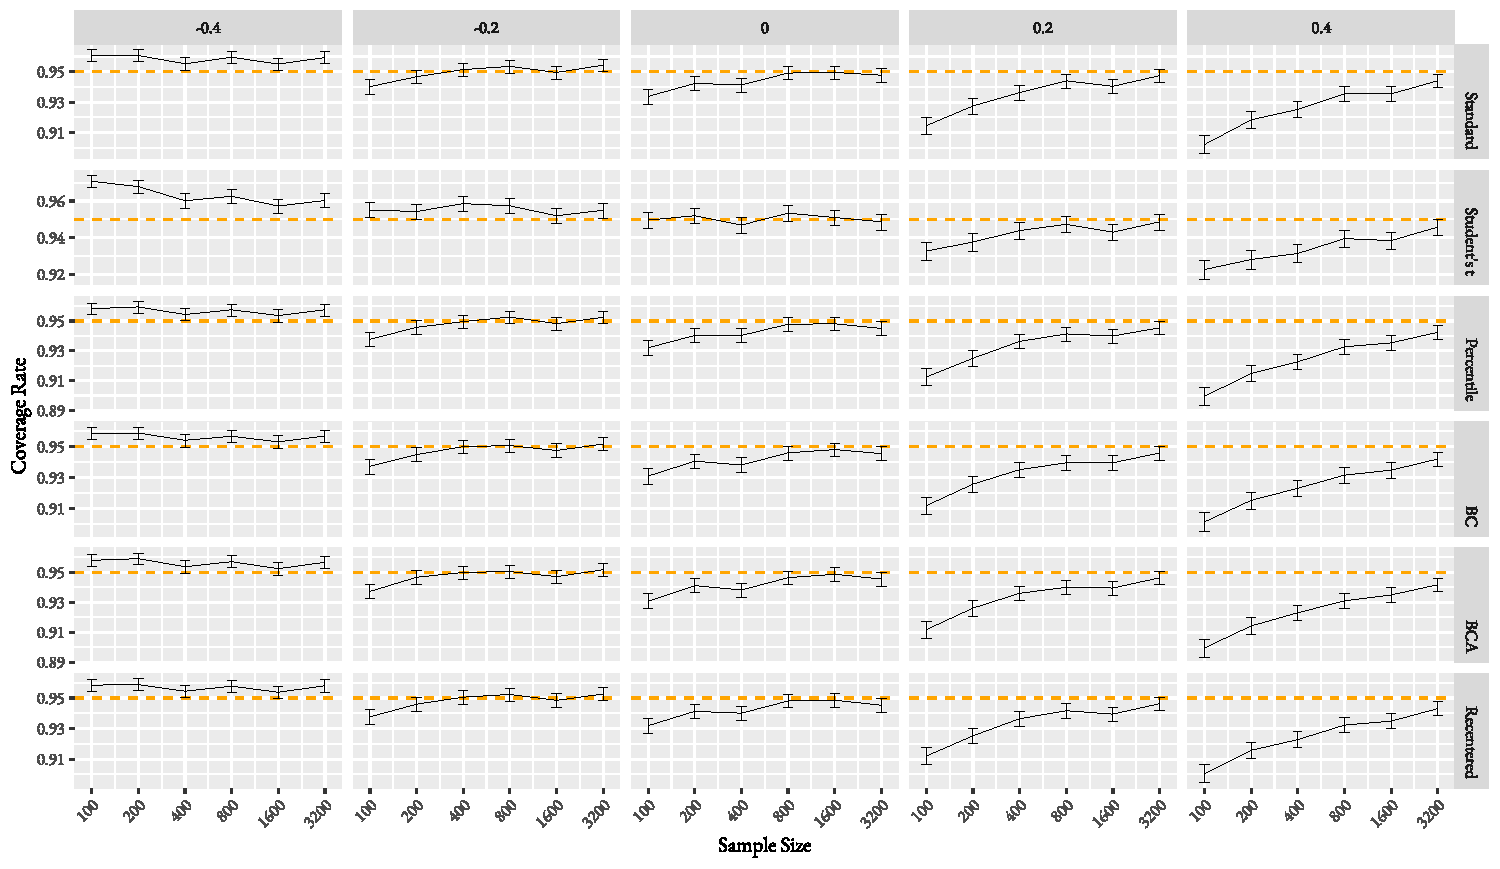
\includegraphics[width=\textwidth]{figures/plot_norm_mu_1}
  \caption{Empirical coverage rates of different 95\% block bootstrap CIs for
    the marginal mean $\mu$ of an AR(1) process with a marginal standard 
    normal distribution with AR coefficient
    $\phi \in \{-0.4, 0.2, 0, 0.2, 0.4\}$ and series length
    $n \in \{100, 200, 400, 800, 1600, 3200\}$ based on 10,000 replicates of
    block bootstrap with $l = \lceil n^{1/3} \rceil$. The
    error bars represent 95\% CIs of the real coverage rates.}
  \label{fig:mu1}
\end{figure}


\begin{figure}[bp]
  \centering
  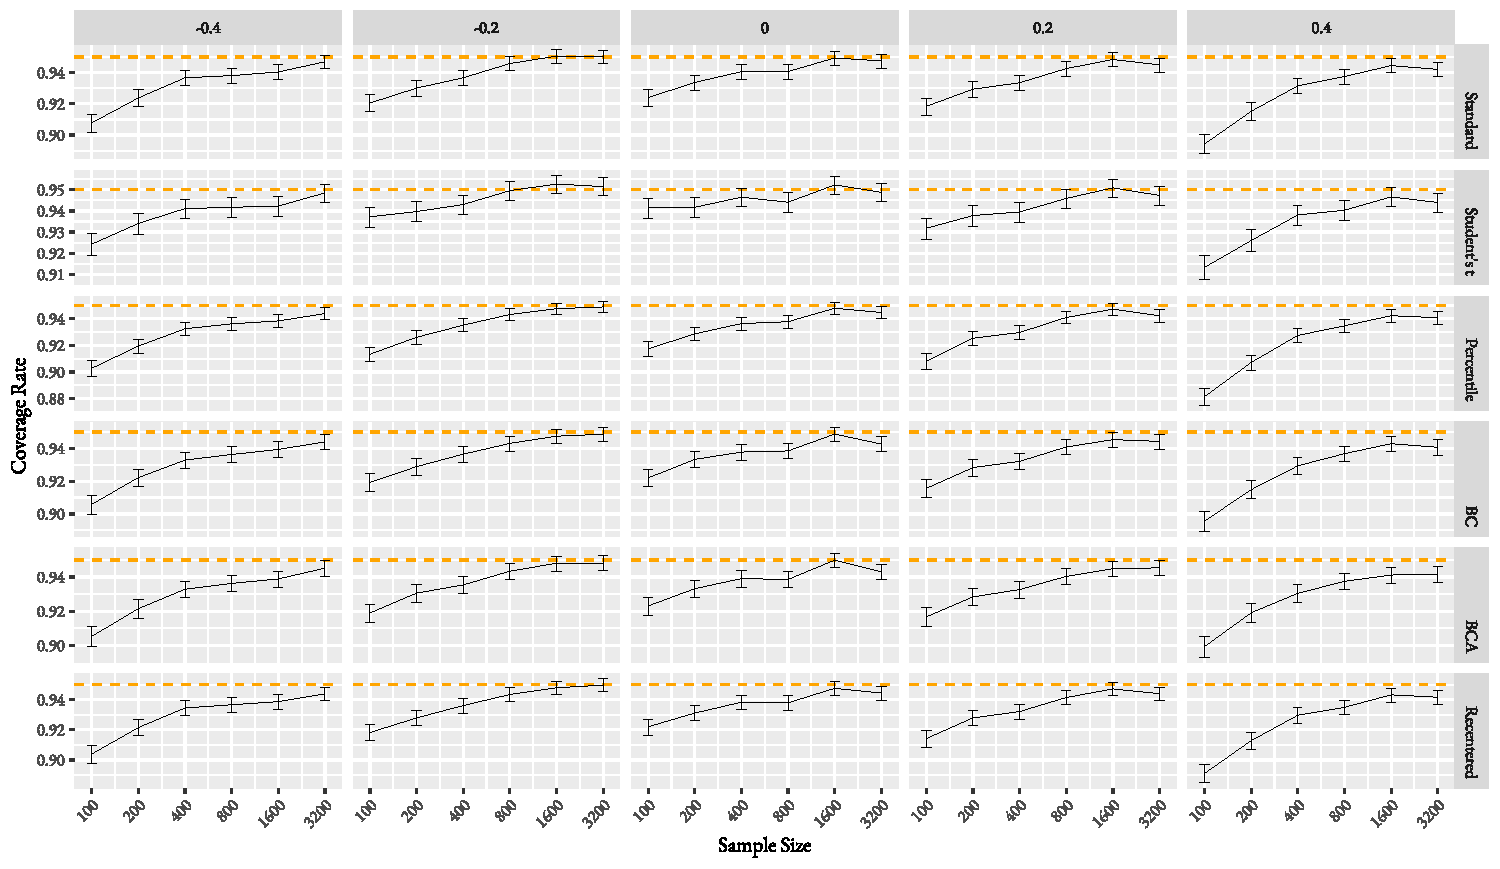
\includegraphics[width=\textwidth]{figures/plot_norm_sigma_1}
  \caption{Empirical coverage rates of different 95\% block bootstrap CIs for
    the marginal standard deviation $\sigma_x$ of an AR(1) process with a
    marginal standard normal distribution with AR 
    coefficient $\phi \in \{-0.4, 0.2, 0, 0.2, 0.4\}$ and series length 
    $n \in \{100, 200, 400, 800, 1600, 3200\}$ based on 10,000 replicates of
    block bootstrap with $l = \lceil n^{1/3} \rceil$. The 
    error bars represent 95\% CIs of the real coverage rates.}
  \label{fig:sigma1}
\end{figure}


\begin{figure}[tbp]
  \centering
  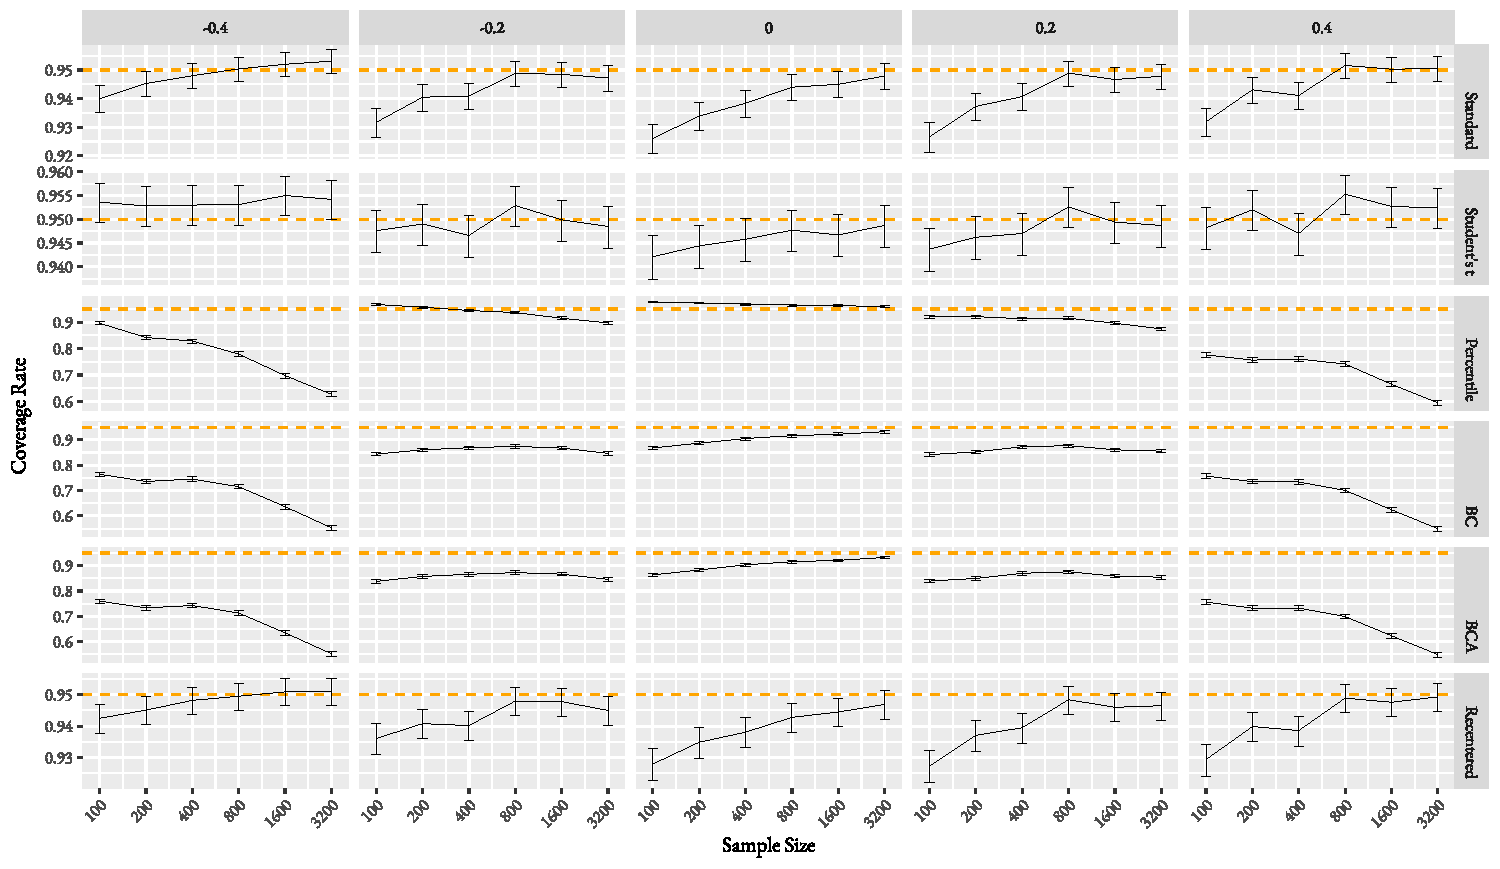
\includegraphics[width=\textwidth]{figures/plot_norm_phi_1}
  \caption{Empirical coverage rates of different 95\% block bootstrap CIs for 
    the first-order autocorrelation coefficient $\phi$ of an AR(1) process with 
    a marginal standard normal distribution with 
    $\phi \in \{-0.4, 0.2, 0, 0.2, 0.4\}$ and series length
    $n \in \{100, 200, 400, 800, 1600, 3200\}$ based on 10,000 replicates of
    block bootstrap with $l = \lceil n^{1/3} \rceil$. The
    error bars represent 95\% CIs of the real coverage rates.}
  \label{fig:phi1}
\end{figure}


\subsection*{Normal Marginal Distribution}
For estimating the mean parameter~$\mu$, \textbf{Figure~\ref{fig:mu1}} suggests 
that all methods eventually approach correct coverage of $\mu$ as sample size 
increases. Student's $t$ CIs appear to need the smallest sample size to achieve 
correct coverage, except for samples with strong negative dependence, in which 
case, they actually over-cover $\mu$ for smaller sample sizes. For instance, for 
a sample with $n = 100$ and $\phi = -0.4$, the lower bound for a Students $t$ 
CI's coverage of $\mu$ is greater than 95\%, whereas the coverage intervals for 
other methods contain 95\%. The standard normal, percentile, BC, and BCA, and 
recentered percentile CIs require similar sample sizes to recover $\mu$ at the 
nominal level for all combinations of $n$ and $\phi$. All methods seem to 
require a smaller sample to recover $\mu$ at the nominal rate when dealing with 
negative dependence versus positive dependence. For example, BC CIs recover 
$\mu$ for $n \geq 100$ when $\phi = -0.2$, but they only recover $\mu$ for 
$n \geq 800$ when $\phi = 0.2$. In addition, as a negative dependence gets 
stronger, holding everything else equal, coverage increases, which lead to the 
Student $t$ CI's aforementioned over-coverage. As a positive dependence gets 
stronger, holding everything else equal, coverage decreases, and a larger sample 
is necessary to recover~$\mu$. A possible explanation for this is that if a 
stationary series has a positive 
autocorrelation, the effective sample
size is decreased, whereas is a series has a negative autocorrelation, the
effective sample size is increased. Additionally, this seems to have a 
greater effect on the the estimation of the location parameter versus that
of the scale parameter or temporal dependence parameter.


CIs for $\mu$ exhibit coverage rates quite close to 1 for $\phi = -0.4$, and
as stated before, the Wald-type CI is known to have undercoverage in such 
situations.
Figure~\ref{fig:norm_mu_1_cp} shows the same coverage rates using exact 
Clopper-Pearson intervals to verify that it is the choice of Wald interval
does not cause undercoverage of the coverage rate. Indeed, the widths of the
exact proportion CIs do not seem to differ heavily from the Wald-type CIs.

\begin{figure}[tbp]
  \centering
  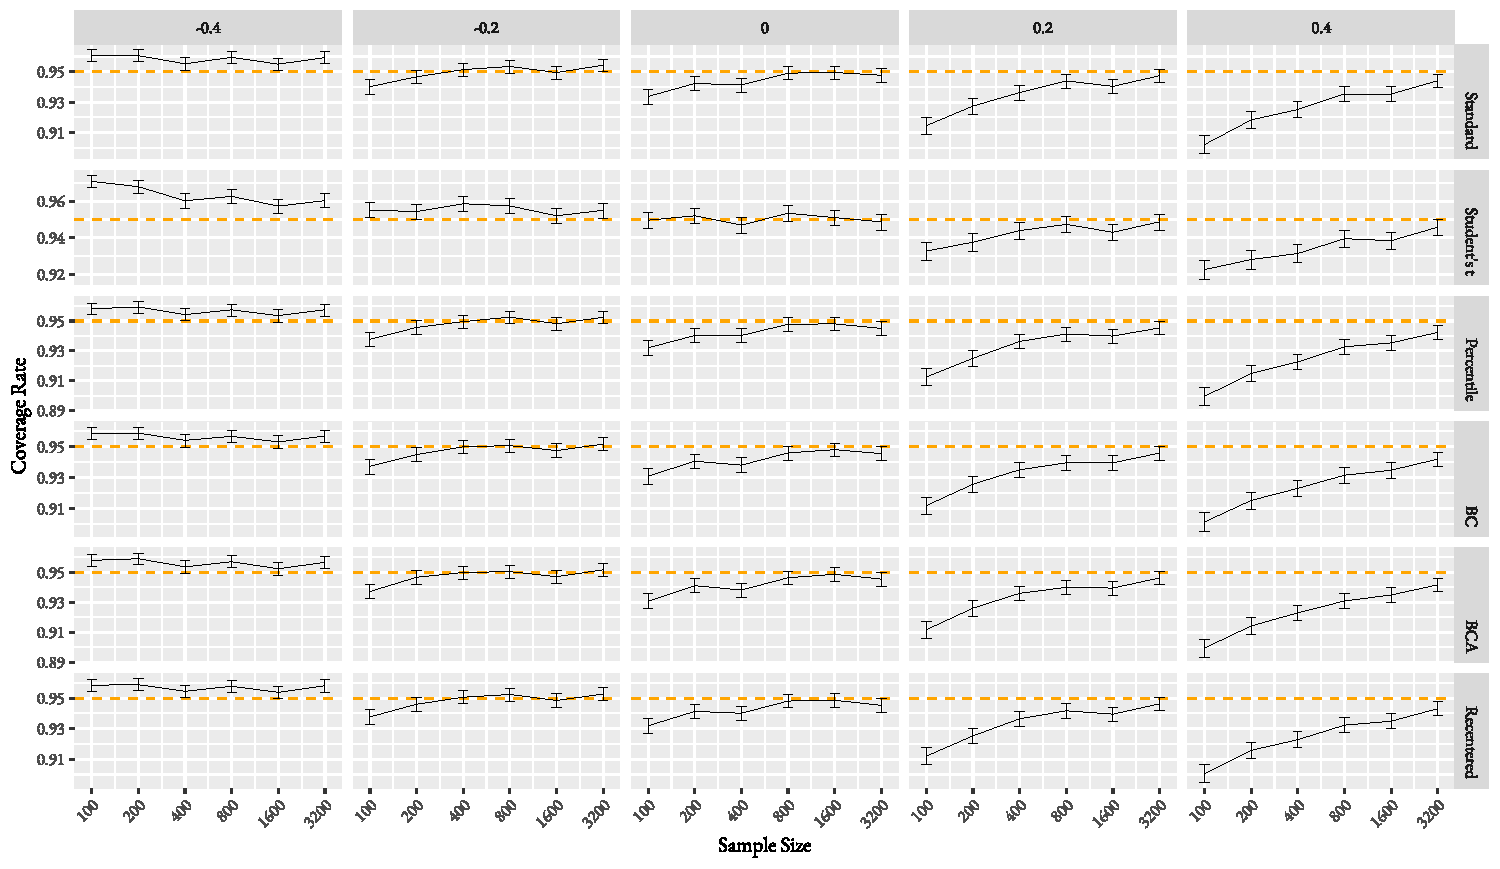
\includegraphics[width=\textwidth]{figures/plot_norm_mu_1_cp}
  \caption{Empirical coverage rates of different 95\% block bootstrap CIs 
    for
    the marginal mean $\mu$ of an AR(1) process with a marginal standard 
    normal distribution with AR coefficient
    $\phi \in \{-0.4, 0.2, 0, 0.2, 0.4\}$ and series length
    $n \in \{100, 200, 400, 800, 1600, 3200\}$ based on 10,000 replicates of
    block bootstrap with $l = \lceil n^{1/3} \rceil$. The
    error bars represent 95\% exact CIs of the real coverage rates.}
  \label{fig:norm_mu_1_cp}
\end{figure}

For estimating the standard deviation parameter~$\sigma_x$,
\textbf{Figure~\ref{fig:sigma1}} suggests that every method can reach nominal 
coverage of $\sigma_x$ if the sample is large enough, but for a given $n$ and 
$\phi$, coverage of $\sigma_x$ will be lower than coverage of $\mu$ in general.
Like $\mu$, $\sigma_x$ can be covered by Student $t$ CIs with smaller sample 
sizes when compared to other methods. Unlike $\mu$, there is no over-coverage 
issue for $\sigma_x$ when $\phi = -0.4$. Standard normal, percentile, BC, BCA, and 
recentered percentile CIs again have similar performance. All methods seem to 
have slightly higher coverage of $\sigma_x$ when $\phi$ is negative versus when 
$\phi$ is positive. Regardless of the sign, coverage of $\sigma_x$ gets worse as 
the strength of the temporal dependence increases.


For estimating the autocorrelation parameter~$\phi$, 
\textbf{Figure~\ref{fig:phi1}} suggests that while standard normal, Student's $t$, and 
recentered percentile CIs do approach correct coverage as sample size increases, 
percentile, BC, and BCA CIs deteriorate as sample size increases, especially as 
the strength of the temporal dependence increases. Because of this, only 
standard normal, Student's $t$, and recentered percentile CIs should be considered as 
effective block bootstrap methods to estimate $\phi$. Student's $t$ CIs once 
again can achieve correct coverage with smaller sample sizes when compared to 
standard and recentered percentile CIs which perform similarly. Student's $t$ 
CIs can can recover $\phi$ at the nominal level for $n \geq 100$ when the 
sample's temporal dependence is as strong as 0.4. Coverage appears to be higher 
for all methods when the dependence is negative rather than positive. Whether or 
not the dependence is negative or positive, coverage of $\phi$ seems to increase 
slightly as the absolute value increases for standard normal, Student's $t$, and 
recentered percentile CIs. For the values of $\phi$ observed, there are no 
examples of over-coverage for standard normal, Student's $t$, BC, BCA, or recentered 
percentile CIs. However, percentile CIs appear to over-cover $\phi$ for smaller 
sample sizes when $\phi = -0.2$ and when $\phi = 0$, indicating again that they 
should not be used.


\begin{figure}[tbp]
  \centering
  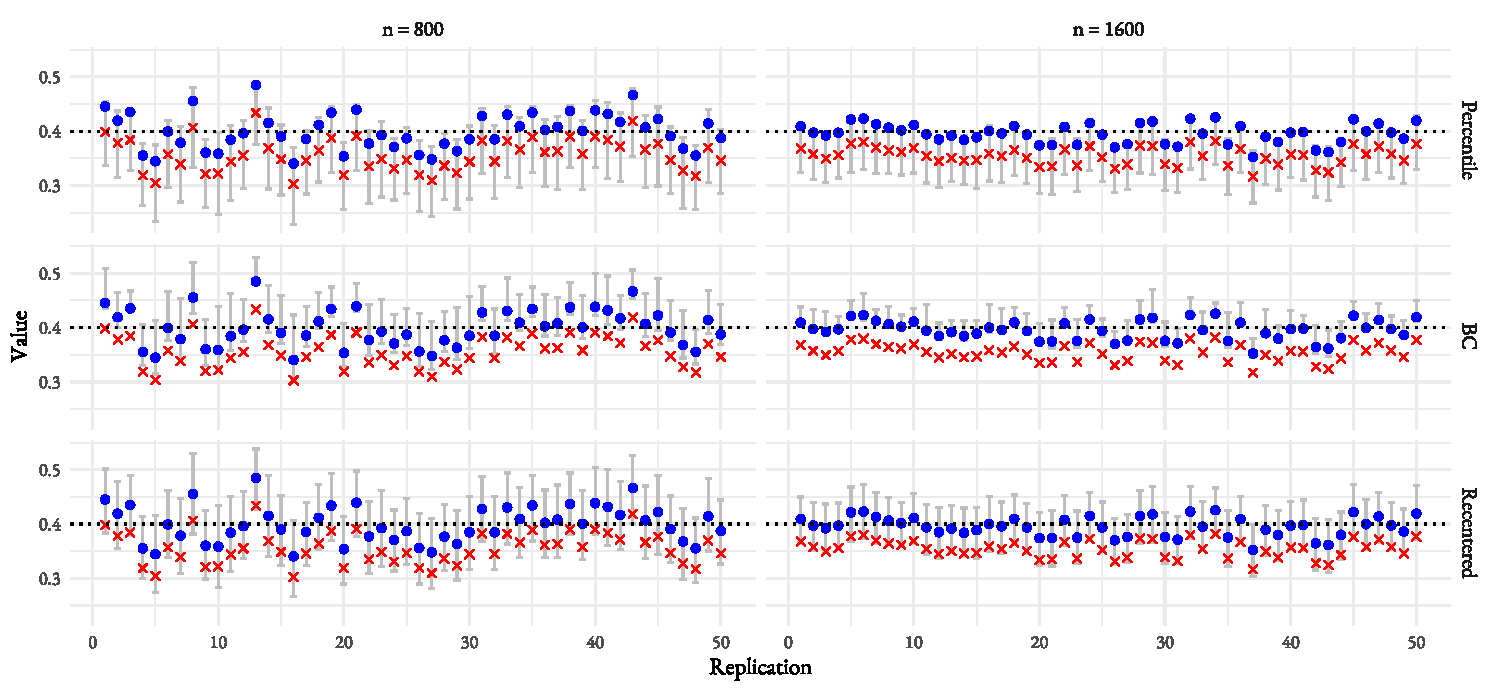
\includegraphics[width=\textwidth]{figures/norm_phi_intervals}
  \caption{50 replicate percentile, BC, and recentered percentile CIs for 
    samples of $n \in \{800, 1600\}$ ($l = \lceil n^{1/3} \rceil$)
    for an AR(1) process with $\phi = 0.4$. For 
    each replicate, the lower and upper bounds of the CIs are displayed, as well 
    as $\hat\theta_n$ (blue circle) and $\bar\theta_n^{B}$ (red cross).}
  \label{fig:npi}
\end{figure}


The outcomes of the $\phi$ estimation raise a natural question about the 
lackluster performance of certain methodologies. To delve into this inquiry, a
set of 50 CIs was generated for each of the percentile, BC, and recentered
percentile  approaches for samples of $n \in \{800, 1600\}$. Illustrated in 
\textbf{Figure~\ref{fig:npi}}, it becomes evident that the percentile-based CIs 
exhibit a notable bias, predominantly manifesting as a substantial 
underestimation of $\phi$ with point estimator $\bar\theta_n^B$, that is, the 
average of $B$ bootstrap point estimates. As the sample size increases from 800 
to 1600, this bias does not vanish while the uncertainty reduces, which explains 
why the coverage rates deteriorate. The bias in $\bar\theta_n^B$ also appears to 
invalidate the bias-correction in the BC bootstrap, leading to the poor 
performance of the BC intervals. The BCA intervals have the same problem as the 
BC intervals in the bias-correction step. The root of the issue appears to be 
that the autocorrelation in the block bootstrap samples is somehow smaller 
compared to that in the original sample. On the other hand, the original point 
estimator $\hat\theta_n$ is asymptotically unbiased. Since the width is based on 
the uncertainty in the bootstrap point estimates $\hat\theta_n^{(b)}$, 
$b = 1, \ldots, B$, the percentile CIs recentered at the original point estimate
$\hat\theta_n$ provide desired coverage.


To summarize, the performance of the CIs depends on the target parameter. When
estimating $\mu$ and $\sigma_x$, any CI will do, although Student's $t$ CIs
perform noticeably better than the others.
However, when estimating $\phi$, the 
choice of method is of utmost importance as to avoid coverage deterioration. 
Coverage rates are acceptable at smaller sample 
sizes when phi is positive versus when phi is negative. In
other words, a larger sample size is generally required to estimate a 
parameter for a sample with a negative $\phi$ versus a positive $\phi$ of the 
same magnitude. In order 
to know if coverage will increase as the strength of the temporal dependence 
increases, one need to know what the parameter of interest is, and in the case 
of $\mu$, the direction of the serial dependence. The BC approach does not seem 
to be correcting bias appropriately when estimating $\phi$. Like the percentile 
method, the recentered percentile method uses the spread from the bootstrap to 
construct the width of the CI. However, the recentered approach, does not 
correct from the original point estimate $\hat\theta_n$.


\begin{figure}[tbp]
  \centering
  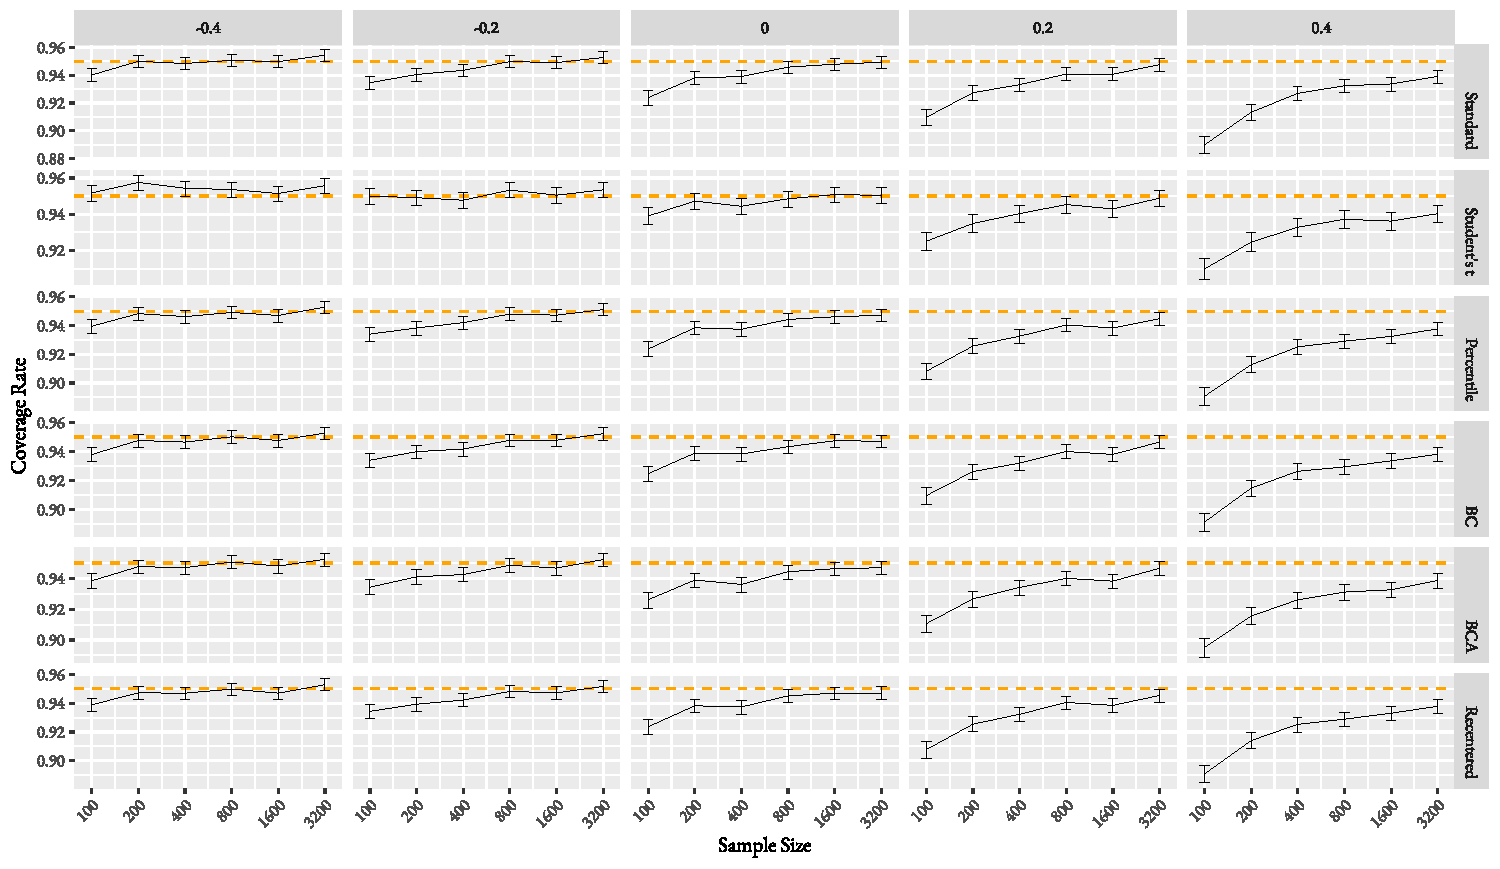
\includegraphics[width=\textwidth]{figures/plot_exp_mu_1}
  \caption{Empirical coverage rates of different 95\% block bootstrap CIs for
    the marginal mean $\mu$ of a stationary series with marginal unit exponential
    distribution obtained by transforming an AR(1) process with
    $\phi \in \{-0.4, 0.2, 0, 0.2, 0.4\}$ with series length
    $n \in \{100, 200, 400, 800, 1600, 3200\}$ based on 10,000 replicates of
    block bootstrap with $l = \lceil n^{1/3} \rceil$. 
    The error bars represent 95\% CIs of the real coverage rates.}
  \label{fig:exp_mu1}
\end{figure}


\begin{figure}[tbp]
  \centering
  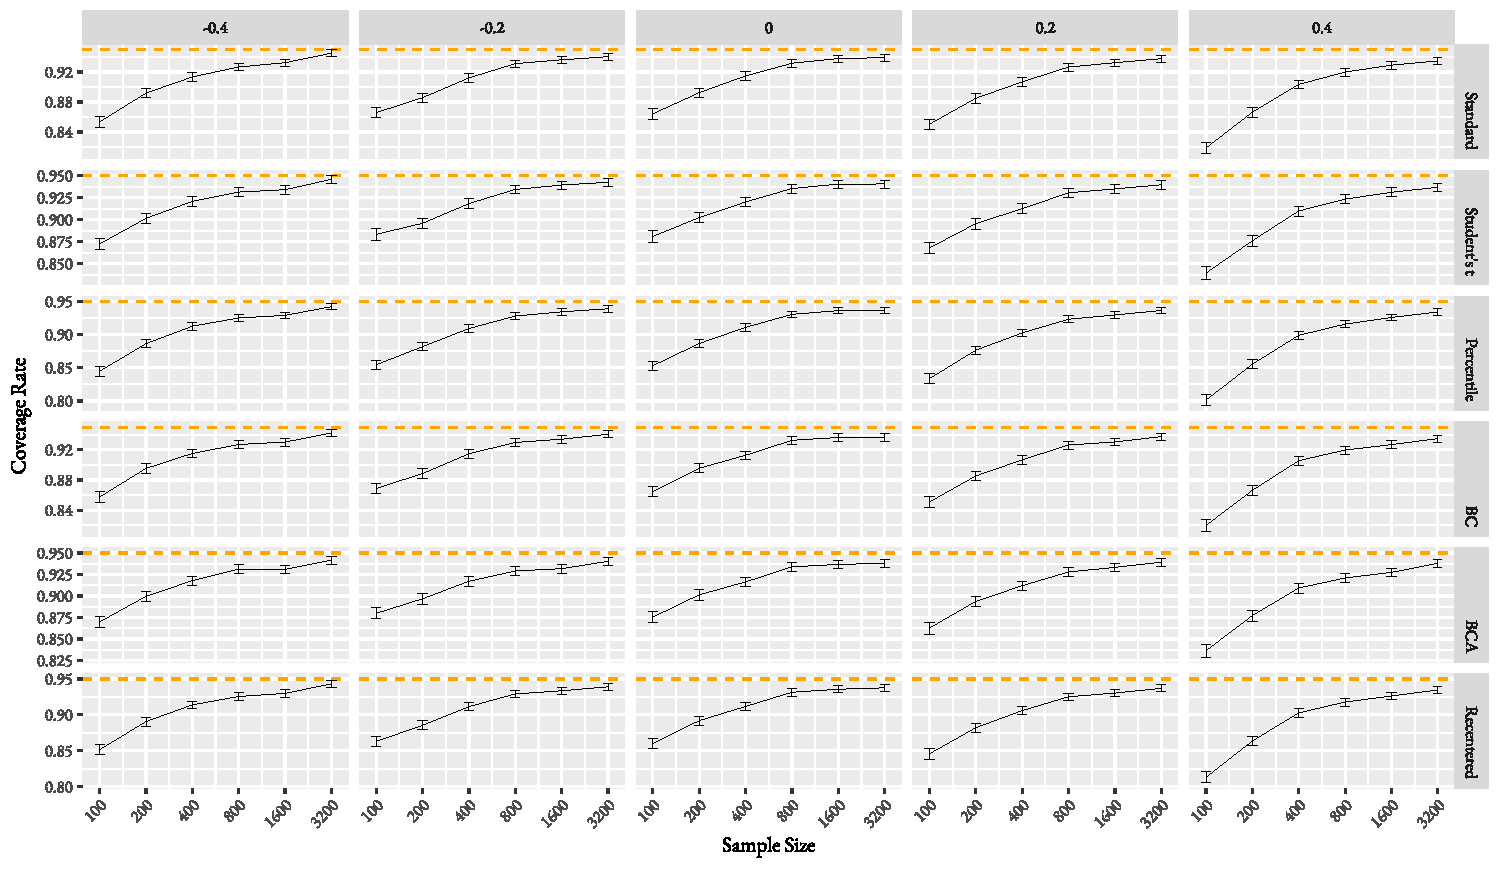
\includegraphics[width=\textwidth]{figures/plot_exp_sigma_1}
  \caption{Empirical coverage rates of different 95\% block bootstrap CIs for
    the marginal standard deviation $\sigma_w$ %\eds{$\sigma_w$?} \mc{addressed}
    of a stationary series with 
    marginal unit exponential distribution obtained by transforming an AR(1) process
    with $\phi \in \{-0.4, 0.2, 0, 0.2, 0.4\}$ with series length 
    $n \in \{100, 200, 400, 800, 1600, 3200\}$ based on 10,000 replicates 
    replicates of
    block bootstrap with $l = \lceil n^{1/3} \rceil$. 
    The error bars represent 95\% CIs of the real coverage rates.}
  \label{fig:exp_sigma1}
\end{figure}


\begin{figure}[tbp]
  \centering
  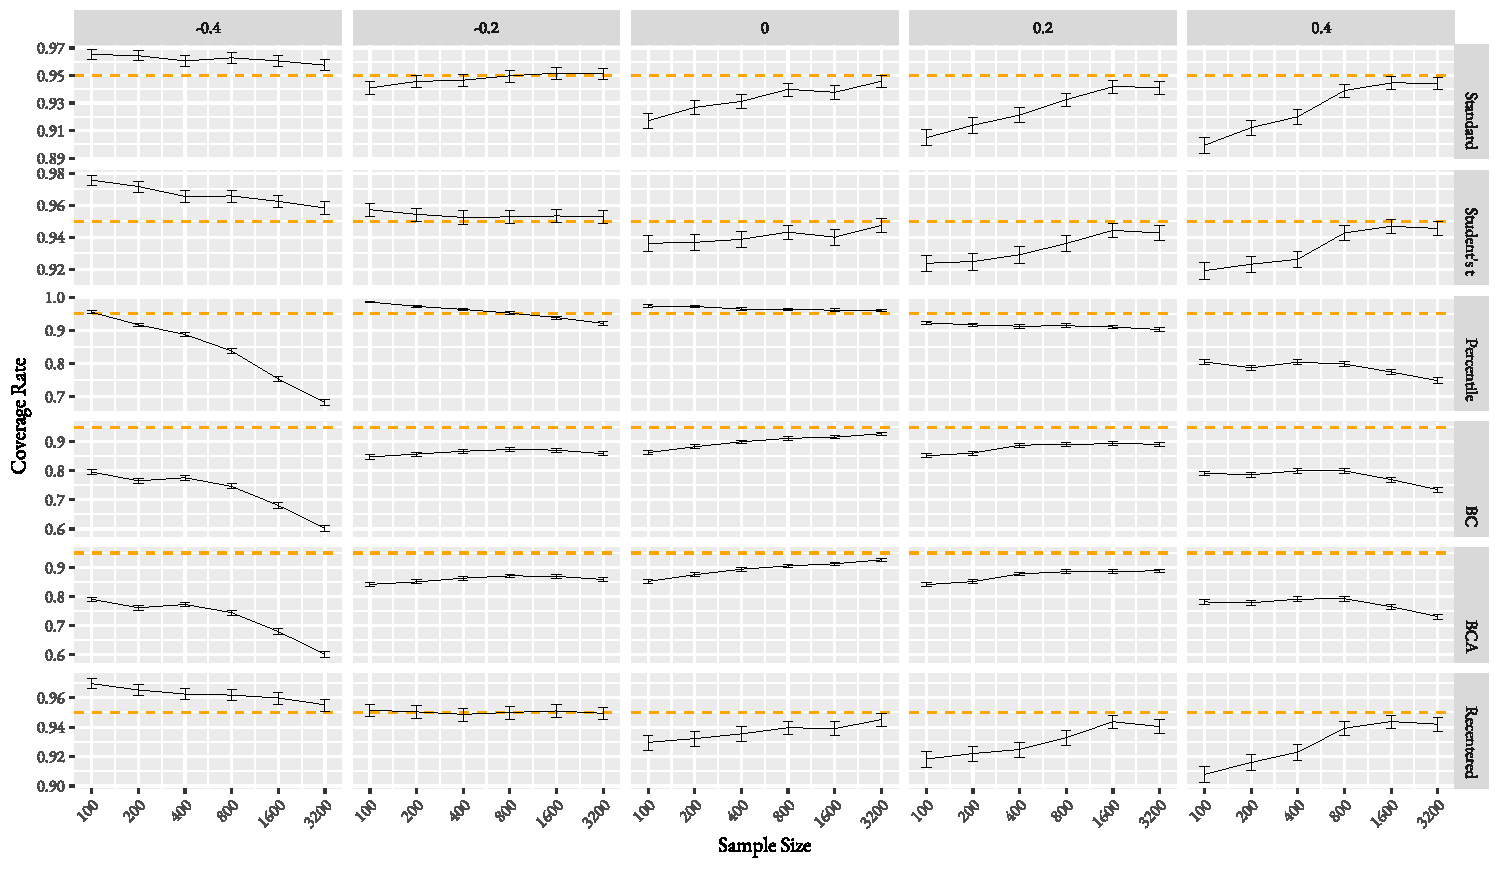
\includegraphics[width=\textwidth]{figures/plot_exp_phi_1}
  \caption{Empirical coverage rates of different 95\% block bootstrap CIs for 
    the first-order autocorrelation coefficient of a stationary series
    with marginal unit exponential distribution obtained by transforming an AR(1) 
    process with 
    $\phi \in \{-0.4, 0.2, 0, 0.2, 0.4\}$ with series length
    $n \in \{100, 200, 400, 800, 1600, 3200\}$ based on 10,000 replicates 
    replicates of
    block bootstrap with $l = \lceil n^{1/3} \rceil$. 
    The error bars represent 95\% CIs of the real coverage rates.}
  \label{fig:exp_phi1}
\end{figure}


\begin{figure}[tbp]
  \centering
  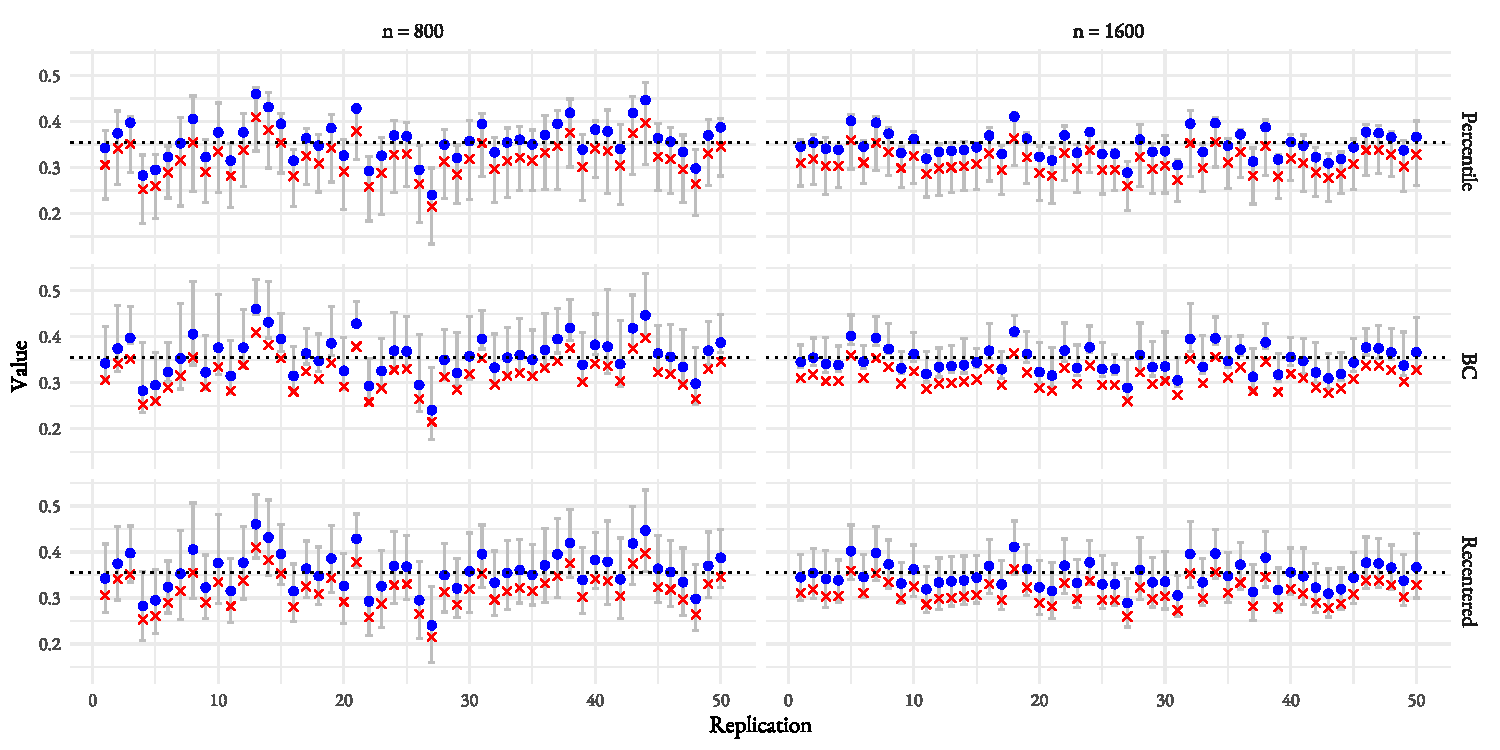
\includegraphics[width=\textwidth]{figures/exp_phi_intervals}
  \caption{50 replicate percentile, BC, and recentered percentile CIs for the
    lag-1 autocorrelation coefficient 0.355 ($\phi = 0.4$)
    of a stationary series with marginal exponential distribution
    obtained by transforming an AR(1) process with $\phi = 0.4$ with
    sample size $n \in \{800, 1600\}$ ($l = \lceil n^{1/3} \rceil$). For 
    each replicate, the lower and upper bounds of the CIs are displayed, as well 
    as $\hat\theta_n$ (blue circle) and $\bar\theta_n^{B}$ (red cross).}
  \label{fig:eri}
\end{figure}

\subsection*{Exponential Marginal Distribution}
For an exponential marginal distribution, the empirical coverage rates for 
$\mu$, $\sigma_w$, %\eds{define $\sigma_w$} 
%\mc{added definitions for $\mu$ and $\sigma_w$ in the above paragraph} 
and 
the lag-1 autocorrelation coefficient, %\mc{replaced $\phi$ here, as I understand
%it, we are not using $\phi$ in reference to the temporal dependence of the 
%exponentially distributed series?}, 
as well as 95\%
confidence intervals of the real coverage are displayed in 
\textbf{Figures~\ref{fig:exp_mu1}--\ref{fig:exp_phi2}}. 
Additionally, a set of 50 CIs are displayed for each of the percentile, 
BC, and recentered percentile approaches for exponentially distributed
samples of $n \in \{800, 1600\}$ with lag-1 autocorrelation coefficient 0.355
($\phi = 0.4$) in Figure~\ref{fig:eri}.


It appears that a greater sample size is generally required for the bootstrap
CIs to cover the mean and standard deviation parameters in the exponential
margin case than in the normal margin case. However, the trends and patterns
discussed in the main text regarding the performance of various methods and
diverse parameters remain consistent. For example, Student's $t$ confidence
intervals still exhibit higher coverage rates in comparison to alternative
methods. Performance continues to be more favorable when temporal dependence is
negative rather than positive. Of particular significance, the 
percentile, BC,
and BCA confidence intervals still display a decline in coverage accuracy for
the lag-1 autocorrelation coefficient as sample size increases as demonstrated
in Figure~\ref{fig:eri}. Both the percentile and BC intervals persist in
manifesting the same bias issue. On the other hand, the recentered percentile
confidence interval continues to be effective in estimating the temporal 
dependence %\mc{replaced $\phi$ again here} 
due to the
inherent unbiasedness of the original point estimator. In sum, the findings for
series that are marginally exponentially distributed closely mirror those
attained for series that are marginally normally distributed.
  
\section*{discussion}
\label{sec:disc}

Block bootstrap is a useful method for estimating parameters of a time series,
from simple parameters like the mean to more complicated temporal dependence
factors. We know theoretically that the block bootstrap procedure will cover a 
parameter of a time series at the nominal level given an infinitely large 
sample, \citep{calhoun2018} so the goal for this study was to find the smallest 
finite sample length 
$n$ of a time series in order for the block bootstrap procedure to recover its 
associated parameters at an acceptable rate. Our analysis relies on the 
assumption that there is a size $n$ large enough for the method to work: that 
is, the method's performance improves as $n$ increases. Out of the six types of 
intervals used in this study, this assumption was found to hold true with 
respect to estimating $\phi$ only for standard normal, Student's $t$, and recentered 
percentile CIs, whereas percentile, BC, and BCA intervals exhibited coverage 
deterioration as $n$ increased. The percentile CI's coverage deterioration can 
be attributed to bias that is not corrected as $n$ increases. Specifically, as 
$n$ increases, the width of the CI decreases, but because the percentile CI 
underestimates $\phi$, the coverage decreases. The BC CI seems to correct the 
bias, but the width of the CI seems to be inconsistent. The acceleration factor 
of the BCA CI seems to fail, as the width of the CI seems to be inconsistent. 


One of the goals of this study was to provide some practical recommendations for 
necessary sample sizes when using block bootstrap to estimate parameters of 
serially dependent data. When using Student's $t$ intervals and $\phi$ is 
unknown, the results of this study suggest that an $n \geq 800$ may be necessary 
for common practice to estimate simpler parameters like $\mu$ or $\sigma_x$. If 
$\phi$ is already known, a lesser $n$ may be adequate to estimate these 
parameters. For lower absolute values of $\phi$, a smaller $n$ is sufficient 
when estimating $\sigma_x$. For negative values of $\phi$, coverage of all 
parameters is higher in general. In fact, Student's $t$ seems to over-cover 
$\mu$ for $\phi = - 0.4$ when using smaller sample sizes, meaning that if $\phi$ 
is known to have a very negative value, another CI may be required. However, in 
real world applications, $\phi$ is more commonly found to be positive, so 
Student's $t$ should still be used if $\phi$ is unknown. Lastly, to estimate 
$\phi$, $n \geq 100$ using the Student's $t$ method may be sufficient. Further
investigation may be necessary to see if there are other interval corrections
that fix the coverage deterioration problem for $\phi$.


This study could be used as a guide for applied statistics courses for students
to generally understand how large of a sample size is sufficient for block
bootstrap to be used versus other inference methods. For undergraduate or 
graduate students, block bootstrap is not typically a part of curriculum, but
the results of this study can easily be used to demonstrate when it is practical 
to use this method. This information could also prove to be useful for research 
using block bootstrap estimation of time series in domains such as econometrics. 
Future studies could investigate the $n$ needed to make inferences about other 
forms of serially dependent data such as a moving average process. One could 
also investigate if there are types of block bootstrap interval construction 
such as $ABC$ or bootstrap-t intervals \citep{efron1993introduction} that could 
more
appropriately recover the parameters of a time series. We discussed some
drawbacks of block bootstrap in the introduction, which could motivate a similar
simulation study for alternatives to block bootstrap, such 
as AR-Sieve bootstrap, \citep{kreiss1992bootstrap} which 
\citet{buhlmann2002bootstraps} finds to be the best for linear time series. 
Lastly, because of its exceptional performance in comparison to the other 
CIs that are not based on bootstrap ``tables", the proposed recentered percentile 
CI would be
an interesting method to study further with different bootstrap schemes.

\section*{Appendix: Simulation Study with $l = \lceil 2n^{1/3} \rceil$}

\textbf{Figures~\ref{fig:mu2}--\ref{fig:phi2}} 
summarizes the empirical coverage rates and the 95\% confidence intervals of the 
real coverage for a standard normal marginal distribution using block bootstrap
with $l = \lceil 2n^{1/3} \rceil$.

\begin{figure}[tbp]
  \centering
  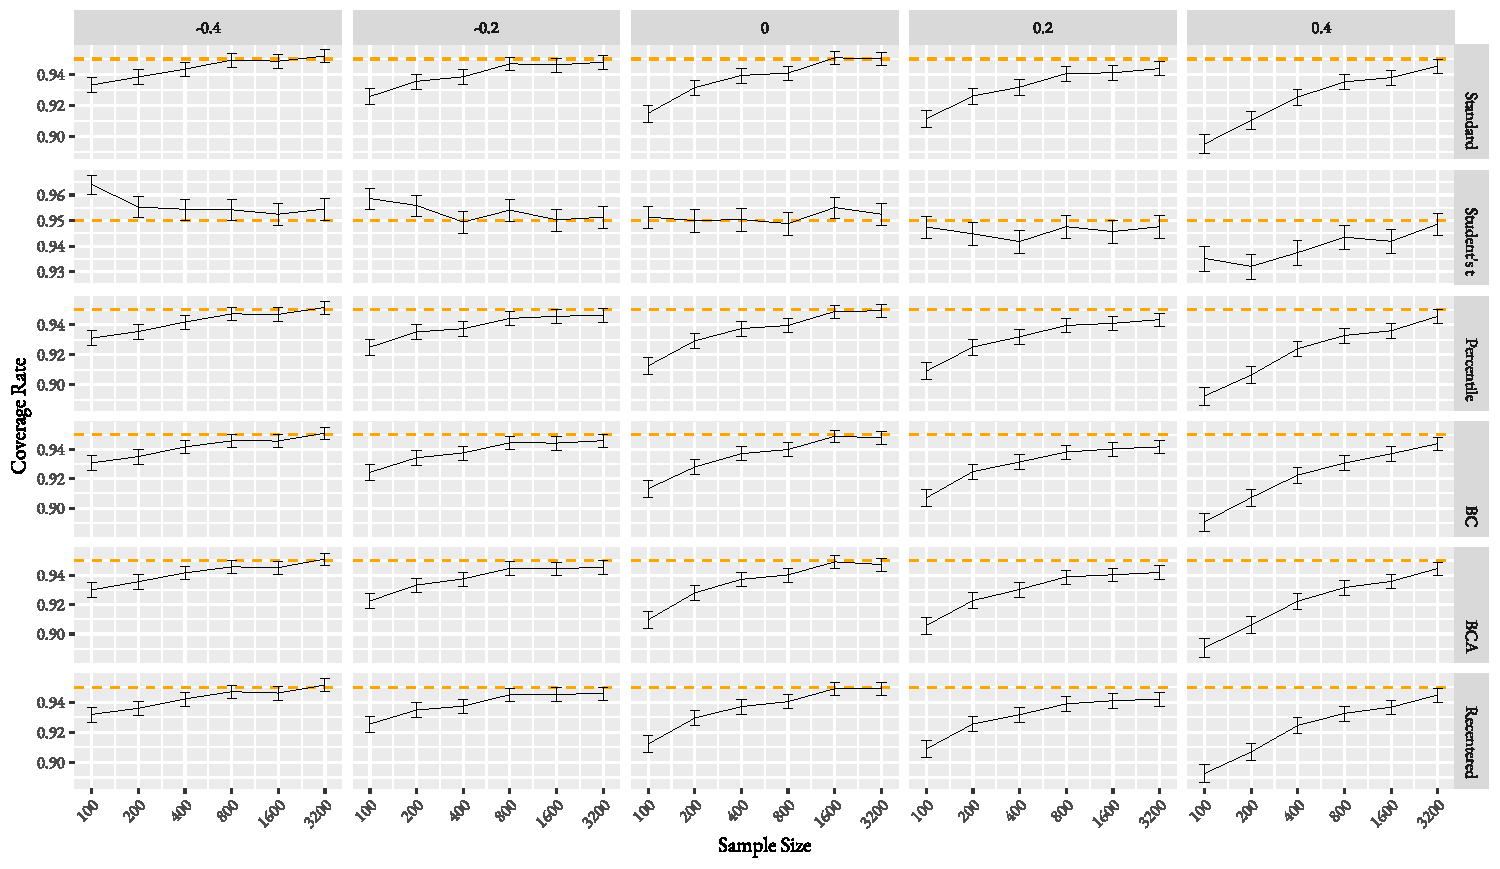
\includegraphics[width=\textwidth]{figures/plot_norm_mu_2}
  \caption{Empirical coverage rates of different 95\% block bootstrap CIs for
    the marginal mean $\mu$ of an AR(1) process with a marginal standard 
    normal distribution with AR coefficient
    $\phi \in \{-0.4, 0.2, 0, 0.2, 0.4\}$ and series length
    $n \in \{100, 200, 400, 800, 1600, 3200\}$ based on 10,000 replicates of
    block bootstrap with $l = \lceil 2n^{1/3} \rceil$. The
    error bars represent 95\% CIs of the real coverage rates.}
  \label{fig:mu2}
\end{figure}


\begin{figure}[bp]
  \centering
  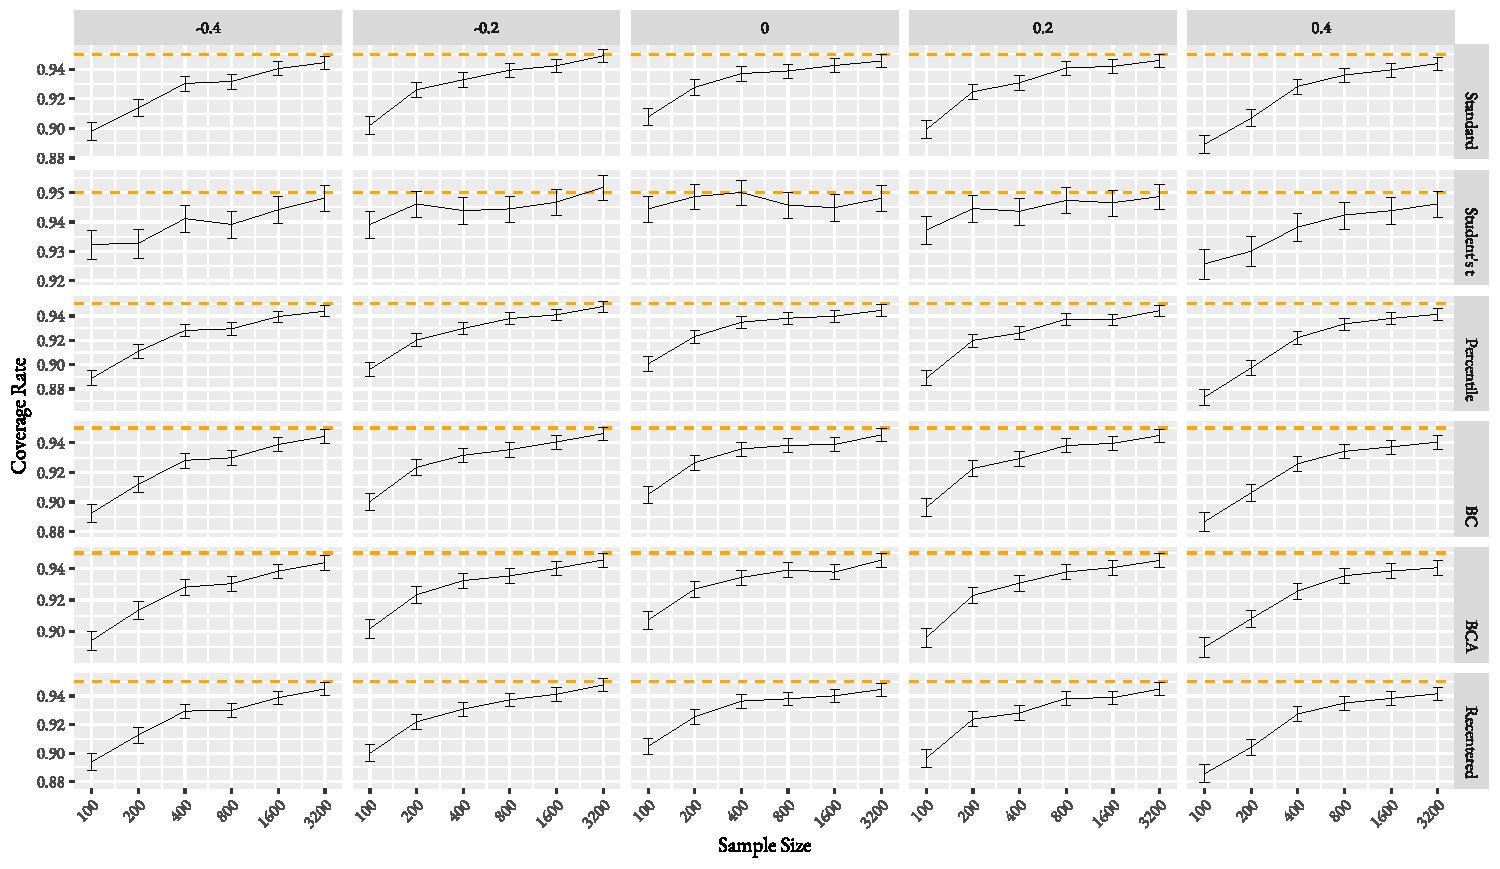
\includegraphics[width=\textwidth]{figures/plot_norm_sigma_2}
  \caption{Empirical coverage rates of different 95\% block bootstrap CIs for
    the marginal standard deviation $\sigma_x$ of an AR(1) process with a
    marginal standard normal distribution with AR 
    coefficient $\phi \in \{-0.4, 0.2, 0, 0.2, 0.4\}$ and series length 
    $n \in \{100, 200, 400, 800, 1600, 3200\}$ based on 10,000 replicates of
    block bootstrap with $l = \lceil 2n^{1/3} \rceil$. The 
    error bars represent 95\% CIs of the real coverage rates.}
  \label{fig:sigma2}
\end{figure}


\begin{figure}[tbp]
  \centering
  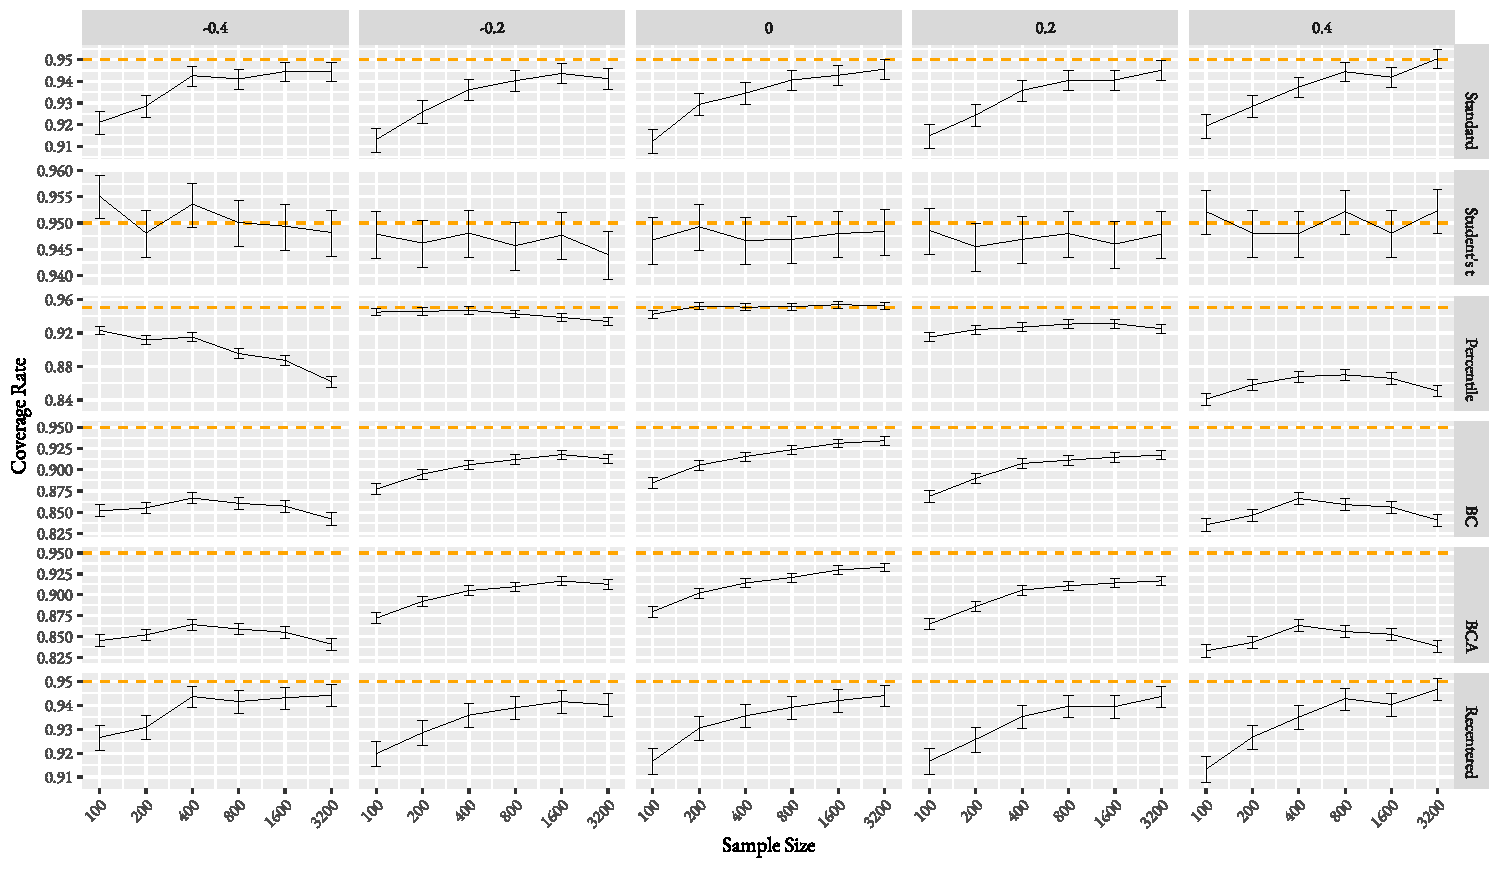
\includegraphics[width=\textwidth]{figures/plot_norm_phi_2}
  \caption{Empirical coverage rates of different 95\% block bootstrap CIs for 
    the first-order autocorrelation coefficient $\phi$ of an AR(1) process with 
    a marginal standard normal distribution with 
    $\phi \in \{-0.4, 0.2, 0, 0.2, 0.4\}$ and series length
    $n \in \{100, 200, 400, 800, 1600, 3200\}$ based on 10,000 replicates of
    block bootstrap with $l = \lceil 2n^{1/3} \rceil$. The
    error bars represent 95\% CIs of the real coverage rates.}
  \label{fig:phi2}
\end{figure}

Based on \textbf{Figure~\ref{fig:mu2}}, for negative autocorrelations, the 
coverage 
rates of $\mu$ appear to be lower when
using $l = \lceil 2n^{1/3} \rceil$. For example, whereas $n = 100$ or 200 
would seem sufficient for most CIs when using $l = \lceil n^{1/3} \rceil$, 
$n = 800$ or 1600 is necessary to capture negative autocorrelations for 
$l = \lceil n^{1/3} \rceil$. Student's $t$ CIs do not seem to be as affected
by this change in $l$: for $\phi = -0.4$ and -0.2, they still overcover $\mu$
for smaller values of $n$. 

\textbf{Figure~\ref{fig:sigma2}} looks very similar to 
\textbf{Figure~\ref{fig:sigma1}}, but coverage rates of $\sigma$ do look 
slightly lower
especially for negative values of $\phi$, although Student's $t$ CIs are again
not as influenced by this change in $l$. A larger sample size seems necessary
when using other CIs to estimate $\sigma$ for $l = \lceil 2n^{1/3} \rceil$.

As shown in \textbf{Figure~\ref{fig:phi2}},
recentered percentile and standard CIs have slightly lower coverage rates when
estimating negative values of $\phi$ with $l = \lceil 2n^{1/3} \rceil$. 
Although it is still a problem, the coverage deterioration appears to be less 
dramatic for BCA,
BC, and percentile CIs.

Aside from these differences, the overall changes
in performance when other experimental factors are changed are the same as
when $l = \lceil n^{1/3} \rceil$.

\textbf{Figures~\ref{fig:exp_mu2}--\ref{fig:exp_phi2}} 
summarizes the empirical coverage rates and the 95\% confidence intervals of the 
real coverage for a exponential marginal distribution using block bootstrap
with $l = \lceil 2n^{1/3} \rceil$.

\begin{figure}[tbp]
  \centering
  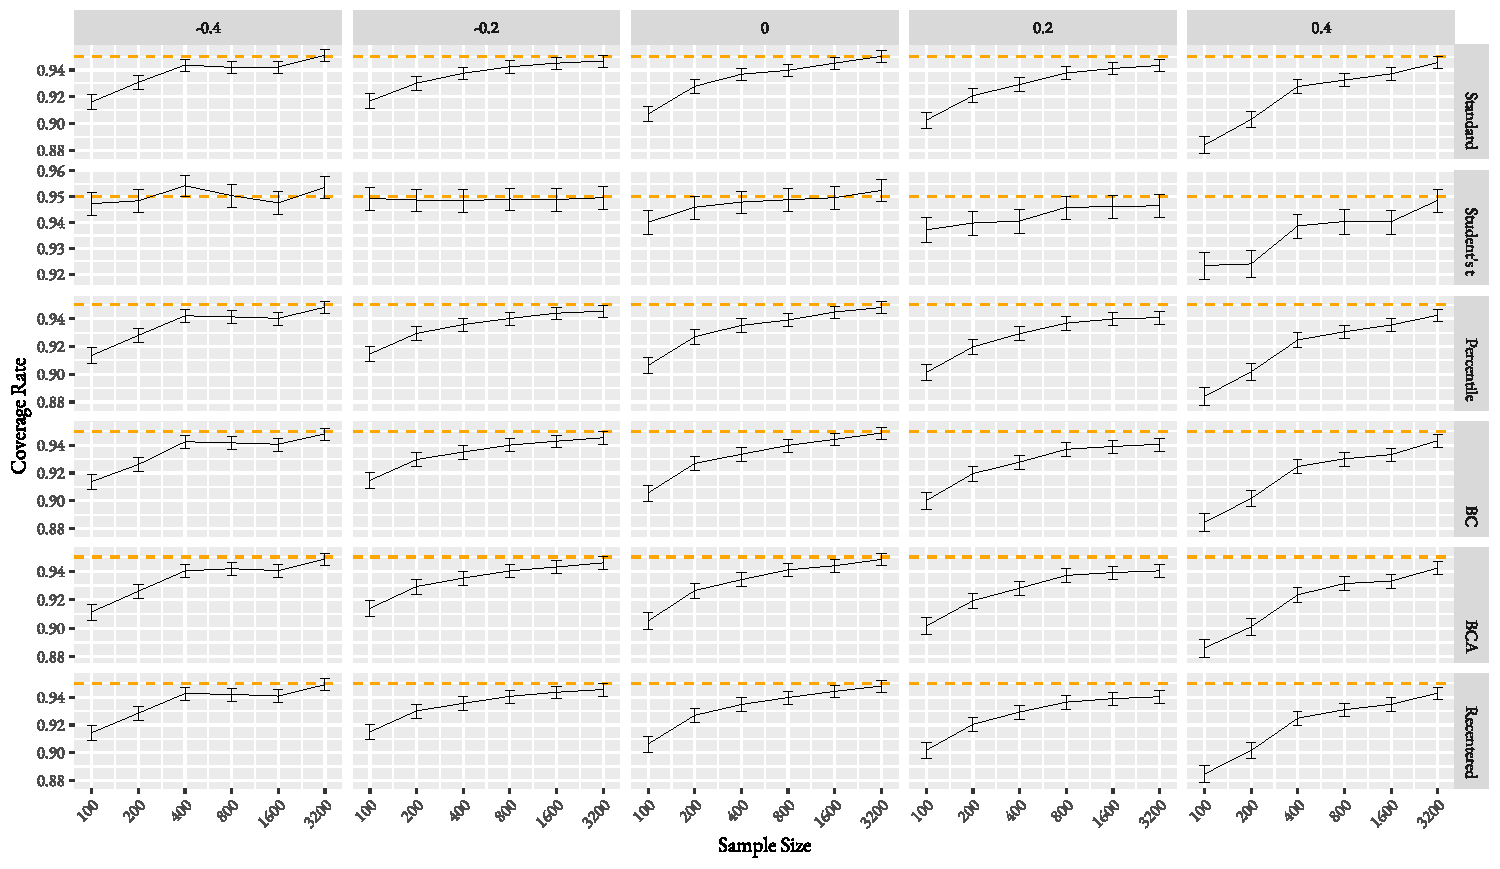
\includegraphics[width=\textwidth]{figures/plot_exp_mu_2}
  \caption{Empirical coverage rates of different 95\% block bootstrap CIs for
    the marginal mean $\mu$ of a stationary series with marginal unit exponential
    distribution obtained by transforming an AR(1) process with
    $\phi \in \{-0.4, 0.2, 0, 0.2, 0.4\}$ with series length
    $n \in \{100, 200, 400, 800, 1600, 3200\}$ based on 10,000 replicates of
    block bootstrap with $l = \lceil 2n^{1/3} \rceil$. 
    The error bars represent 95\% CIs of the real coverage rates.}
  \label{fig:exp_mu2}
\end{figure}


\begin{figure}[tbp]
  \centering
  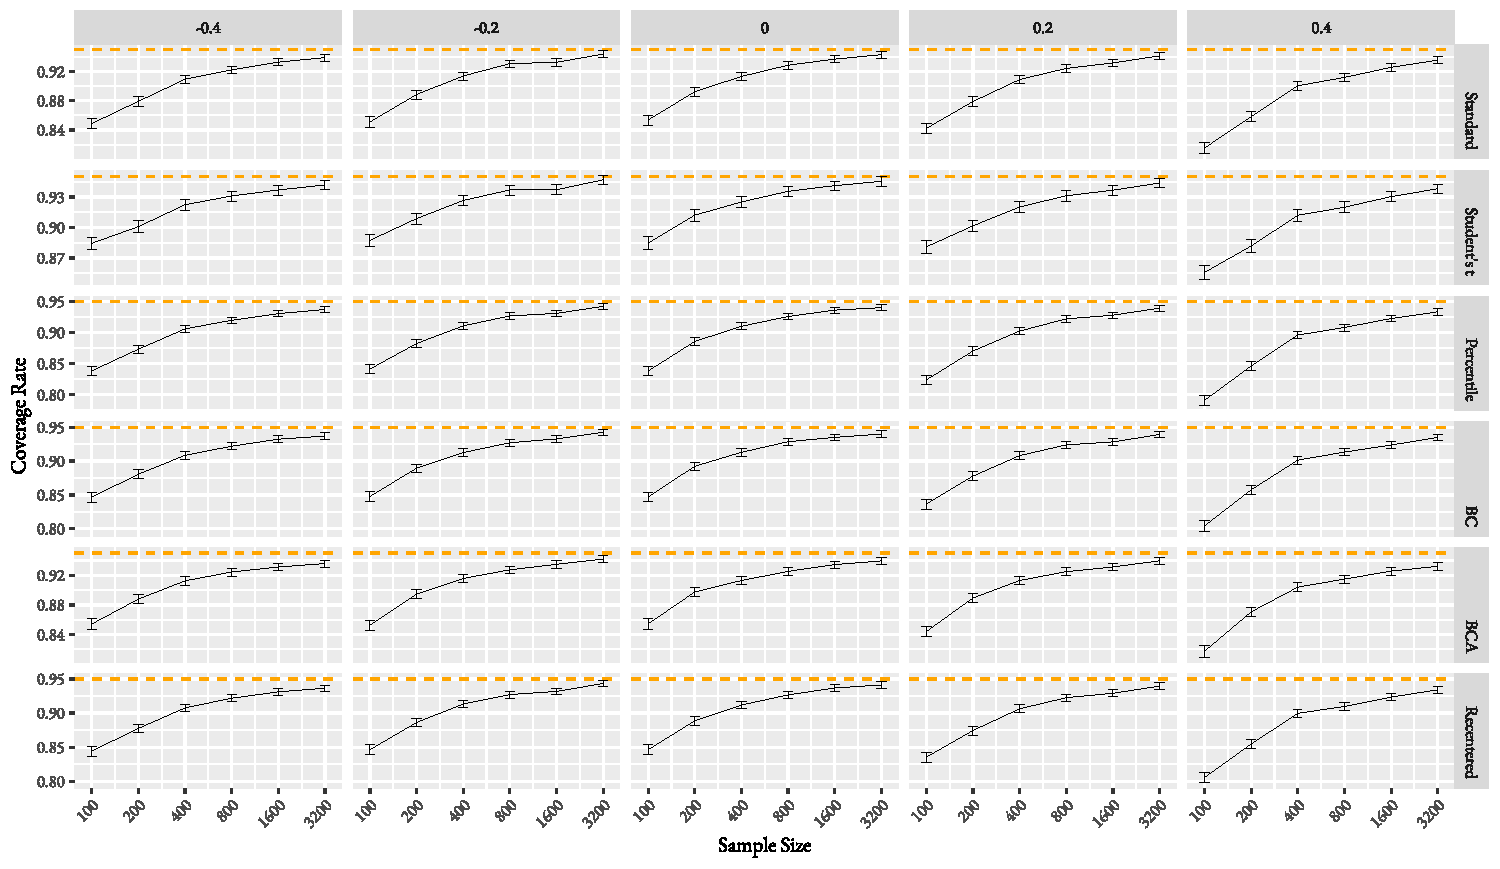
\includegraphics[width=\textwidth]{figures/plot_exp_sigma_2}
  \caption{Empirical coverage rates of different 95\% block bootstrap CIs for
    the marginal standard deviation $\sigma_w$ %\eds{$\sigma_w$?} \mc{addressed}
    of a stationary series with 
    marginal unit exponential distribution obtained by transforming an AR(1) process
    with $\phi \in \{-0.4, 0.2, 0, 0.2, 0.4\}$ with series length 
    $n \in \{100, 200, 400, 800, 1600, 3200\}$ based on 10,000 replicates 
    replicates of
    block bootstrap with $l = \lceil 2n^{1/3} \rceil$. 
    The error bars represent 95\% CIs of the real coverage rates.}
  \label{fig:exp_sigma2}
\end{figure}


\begin{figure}[tbp]
  \centering
  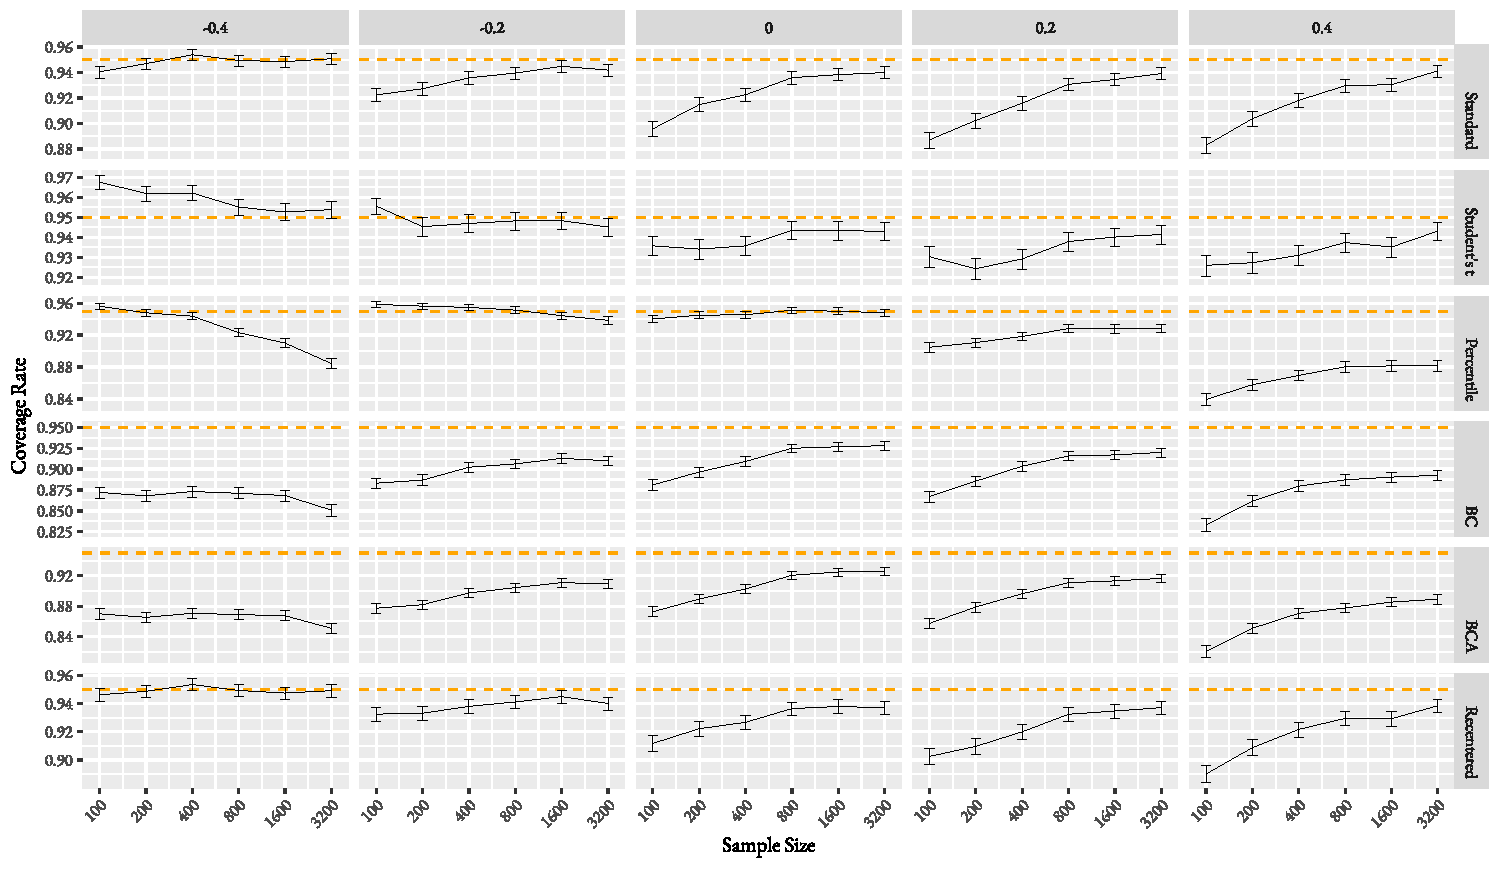
\includegraphics[width=\textwidth]{figures/plot_exp_phi_2}
  \caption{Empirical coverage rates of different 95\% block bootstrap CIs for 
    the first-order autocorrelation coefficient of a stationary series
    with marginal unit exponential distribution obtained by transforming an AR(1) 
    process with 
    $\phi \in \{-0.4, 0.2, 0, 0.2, 0.4\}$ with series length
    $n \in \{100, 200, 400, 800, 1600, 3200\}$ based on 10,000 replicates 
    replicates of
    block bootstrap with $l = \lceil 2n^{1/3} \rceil$. 
    The error bars represent 95\% CIs of the real coverage rates.}
  \label{fig:exp_phi2}
\end{figure}

For a stationary series with a marginal exponential distribution, altering the 
block size results in the same 
changes in performance of different CIs.
 
\bibliographystyle{unsrtnat}
\bibliography{citations}

\end{document}
